\chapter{Elaboration: Analysis and Architecture}
\label{chap:elaboration}

\section{Introduction}

The elaboration phase analyses the requirements of Chapter~\ref{chap:inception} and builds the architecture on which the construction iterations grow. This chapter says what the system is made of and why: the technical choices, the overall architecture, the analysis model, the dynamic view of the key use cases, the detection architecture, and the framing of the machine learning problem. It ends with the architecture baseline that the phase delivered, and the risks it reduced. How each part was implemented is described in the iterations of Chapter~\ref{chap:construction}.

\section{Technical choices}
\label{sec:tech-used}

Figure~\ref{fig:tech-logos} shows the technologies used in the project.

\begin{figure}[H]
\centering
\begin{tabular}{ccccc}
\techlogo{dotnet.pdf}{C\# / .NET / WPF} & \techlogo{python.pdf}{Python} & \techlogo{fastapi.pdf}{FastAPI} & \techlogo{sqlite.pdf}{SQLite} & \techlogo{scikitlearn.pdf}{scikit-learn} \\[0.45cm]
\techlogo{pandas.pdf}{pandas} & \techlogo{numpy.pdf}{NumPy} & \techlogo{pytest.pdf}{pytest} & \techlogo{googlegemini.pdf}{Google Gemini} & \techlogo{ollama.pdf}{Ollama} \\[0.45cm]
\techlogo{arduino.pdf}{Arduino} & \techlogo{git.pdf}{Git} & \techlogo{github.pdf}{GitHub} & \techlogo{drawio.pdf}{draw.io} & \techlogo{latex.pdf}{\LaTeX} \\
\end{tabular}
\caption[Technologies used in the project.]{Technologies used in the client, the backend, the machine learning, the tests, the bench rig and the documentation.}
\label{fig:tech-logos}
\end{figure}

The role of each technology is the following:

\begin{itemize}
    \item \textbf{C\# and WPF (.NET Framework 4.8):} \gls{wpf} is the Microsoft framework for native Windows desktop applications, used here with the \gls{mvvm} pattern and the CommunityToolkit.Mvvm library. Its data binding suits a client with many screens and charts, and .NET Framework 4.8 was the target platform of the project.
    \item \textbf{Python, FastAPI, pandas and NumPy:} FastAPI~\cite{fastapi} builds typed \gls{rest} APIs that document themselves, and it works directly with the Python data libraries used for the machine learning. The backend is served by uvicorn.
    \item \textbf{scikit-learn:} The scikit-learn library~\cite{pedregosa2011scikit} provides the Isolation Forests~\cite{liu2008isolation} of the models and the K-Means~\cite{macqueen1967methods} of the first design. Classical methods covered both needs, so no deep learning framework was required.
    \item \textbf{asammdf, cantools and python-can:} The asammdf library reads ASAM \gls{mf4}~\cite{asam_mdf} logs, cantools decodes frames with a \gls{dbc} file, and python-can~\cite{pythoncan} gives one interface to many physical \gls{can} adapters, including the Arduino bridge of our bench rig.
    \item \textbf{SQLite:} An embedded database without a server, enough for a system that runs on one workstation.
    \item \textbf{Google Gemini and Ollama:} They are used only by the explanation module: Gemini in the cloud, Ollama as a local model that works without an internet connection. When neither is available, a rule based template writes the explanation.
    \item \textbf{Development environment:} Visual Studio for the client, a Python virtual environment for the backend, PDFsharp to build the PDF report in C\#, pytest and xUnit for the automated tests, Git and GitHub to version the project, with the large model files in Git LFS, draw.io for the diagrams and MiKTeX for this report. A Windows workstation served for development, training and validation, and a bench rig of two Arduino boards for live capture.
\end{itemize}

\Needspace{657pt}% keep the heading with its float
\section{Overall architecture}
\label{sec:architecture}

\subsection{Logical view in layers}

CANvisionNative runs as two programs on the same machine, a Windows desktop client and a local Python backend, which talk over \gls{http}, as shown in Figure~\ref{fig:overall-arch} below.

The client only talks to the \gls{api} layer, which sends each request to the detection engine or to the data layer, and calls the explanation engine only when the analyst asks for an explanation. We chose this separation so that the detection could be tested through the \gls{api} without the client.

\begin{figure}[H]
\centering
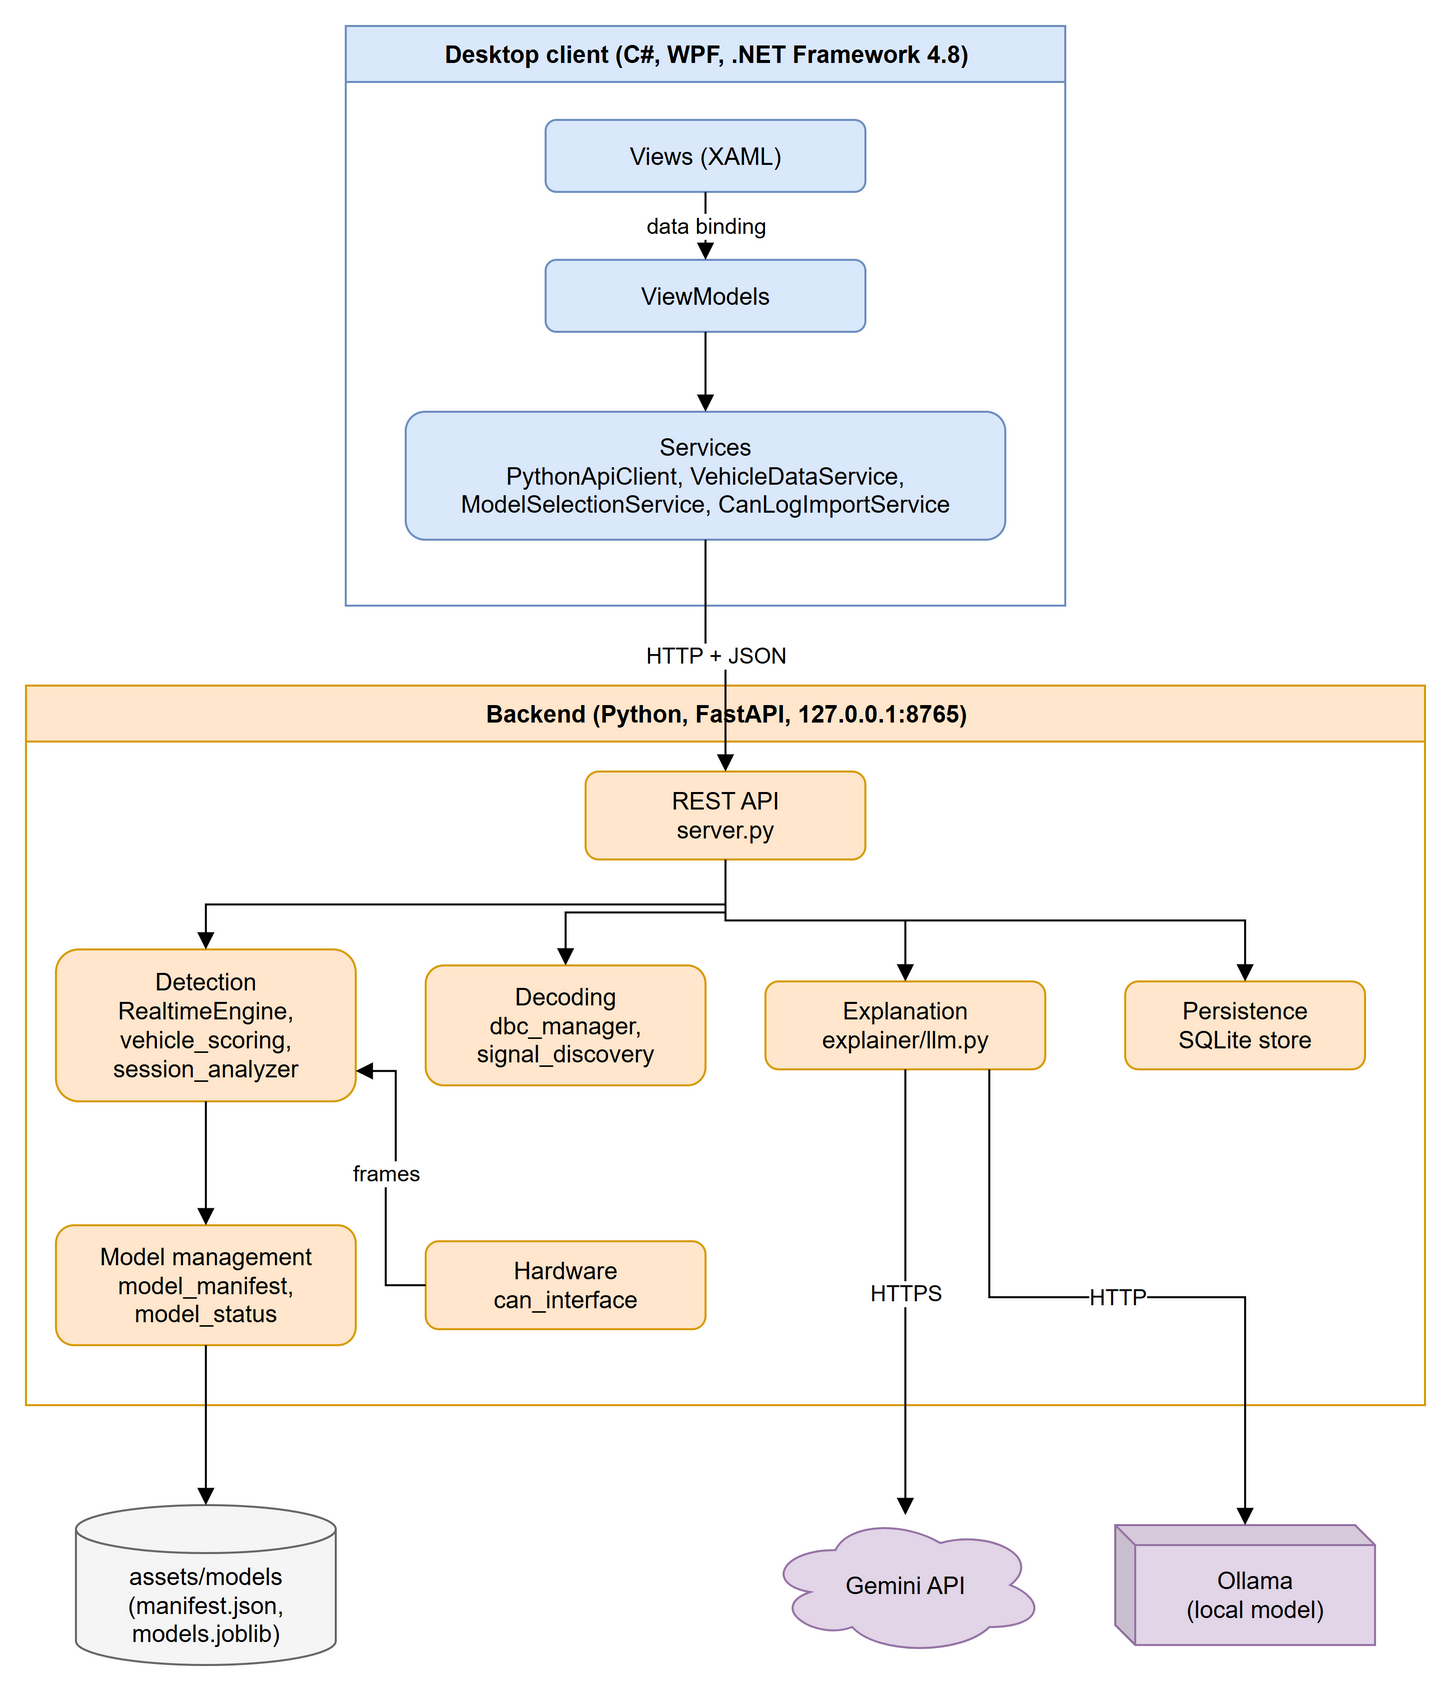
\includegraphics[width=0.8\textwidth]{architecture_overall.png}
\caption{Overall layered architecture of CANvisionNative.}
\label{fig:overall-arch}
\end{figure}

\subsection{Components}
\label{sec:design-backend}

Figure~\ref{fig:components} shows the components and their dependencies. In the client, the views are bound to their ViewModels, which go through a layer of client services to reach the backend. In the backend, the \gls{rest} \gls{api} is the only entry point. It starts the offline analyzer for whole recordings, the replay runner and the hardware interface for frame by frame traffic, and calls the explanation engine and the persistence layer. The replay runner and the hardware interface share the runtime engine, and every component that scores frames obtains its models through the model management component, which reads the model files and their manifests. Long tasks, such as a replay or an offline analysis, run in the background while the client follows their status.

\begin{figure}[H]
\centering
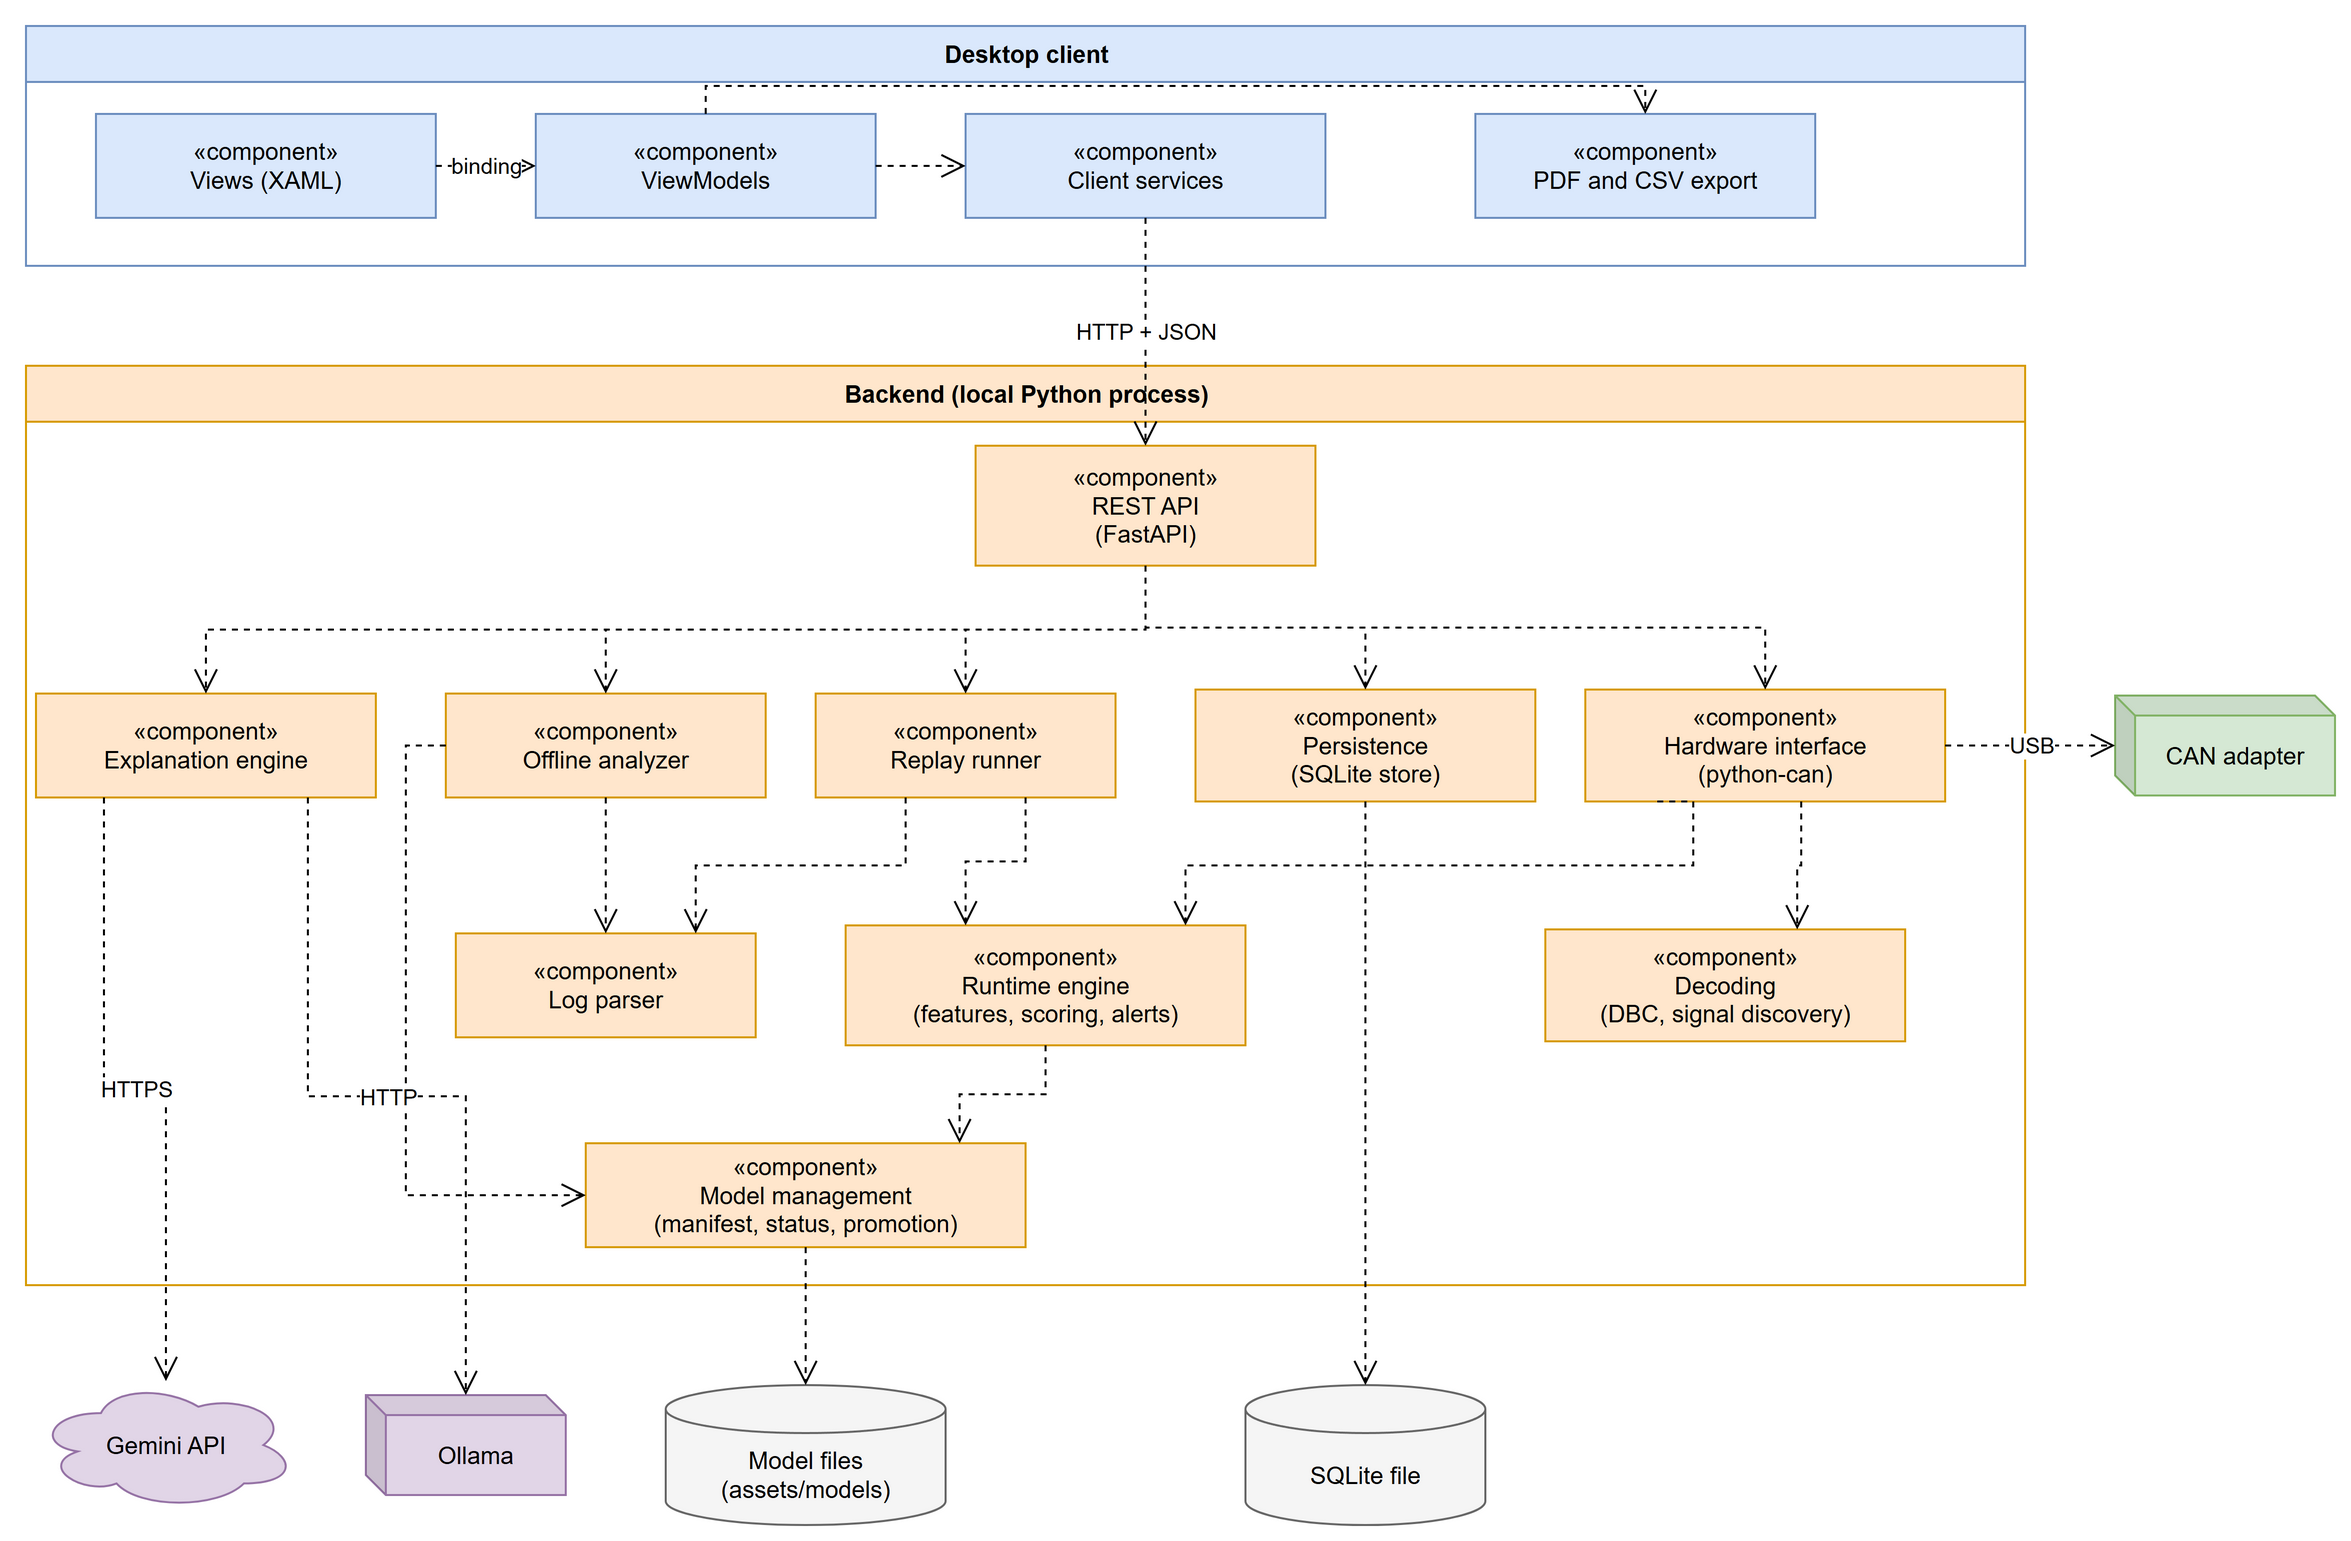
\includegraphics[width=\textwidth]{component_diagram.png}
\caption{Component diagram of the client and the backend.}
\label{fig:components}
\end{figure}

\Needspace{538pt}% keep the heading with its float
\subsection{Client architecture (MVVM)}
\label{sec:design-frontend}

Each screen of the client (Home, Dashboard, Telemetry, Diagnostics, Log Playback, Anomaly Intel and Settings) has a XAML view and its ViewModel; a Hardware Setup screen opens from Home when a live session starts. Two services sit between the ViewModels and the backend (Figure~\ref{fig:frontend-arch}): an \gls{api} client with one method per endpoint, and a data service that keeps the shared state, polls the backend and notifies the screens.

\begin{figure}[H]
\centering
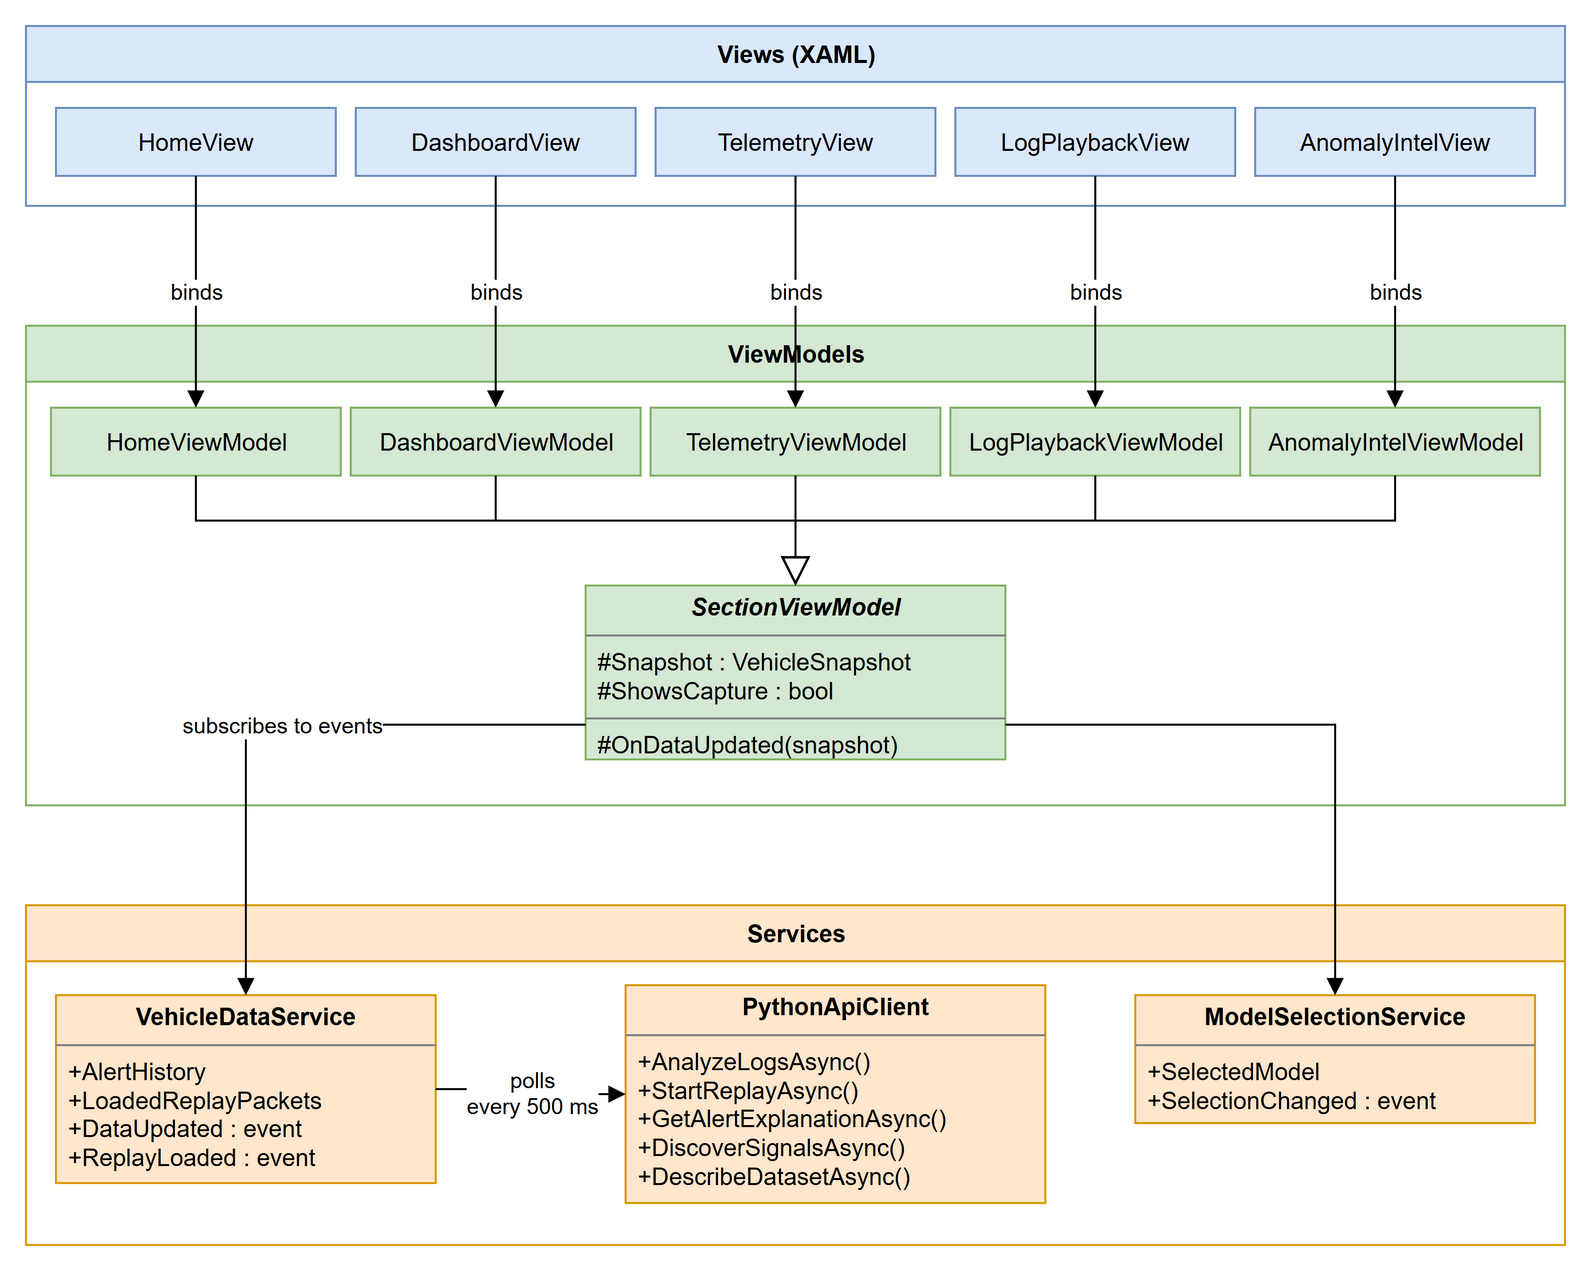
\includegraphics[width=\textwidth]{architecture_frontend.png}
\caption[Frontend architecture of the client.]{Frontend architecture: MVVM views bound to their ViewModels, with two shared services.}
\label{fig:frontend-arch}
\end{figure}

\Needspace{447pt}% keep the text with its float
\Needspace{447pt}% keep the heading with its float
\subsection{Deployment}

Figure~\ref{fig:deployment} shows the deployment. The client and the backend run on the analyst's workstation, next to the SQLite file, the model folder and an optional local Ollama model; Gemini is reached over HTTPS, and the \gls{can} adapter over USB.

\begin{figure}[H]
\centering
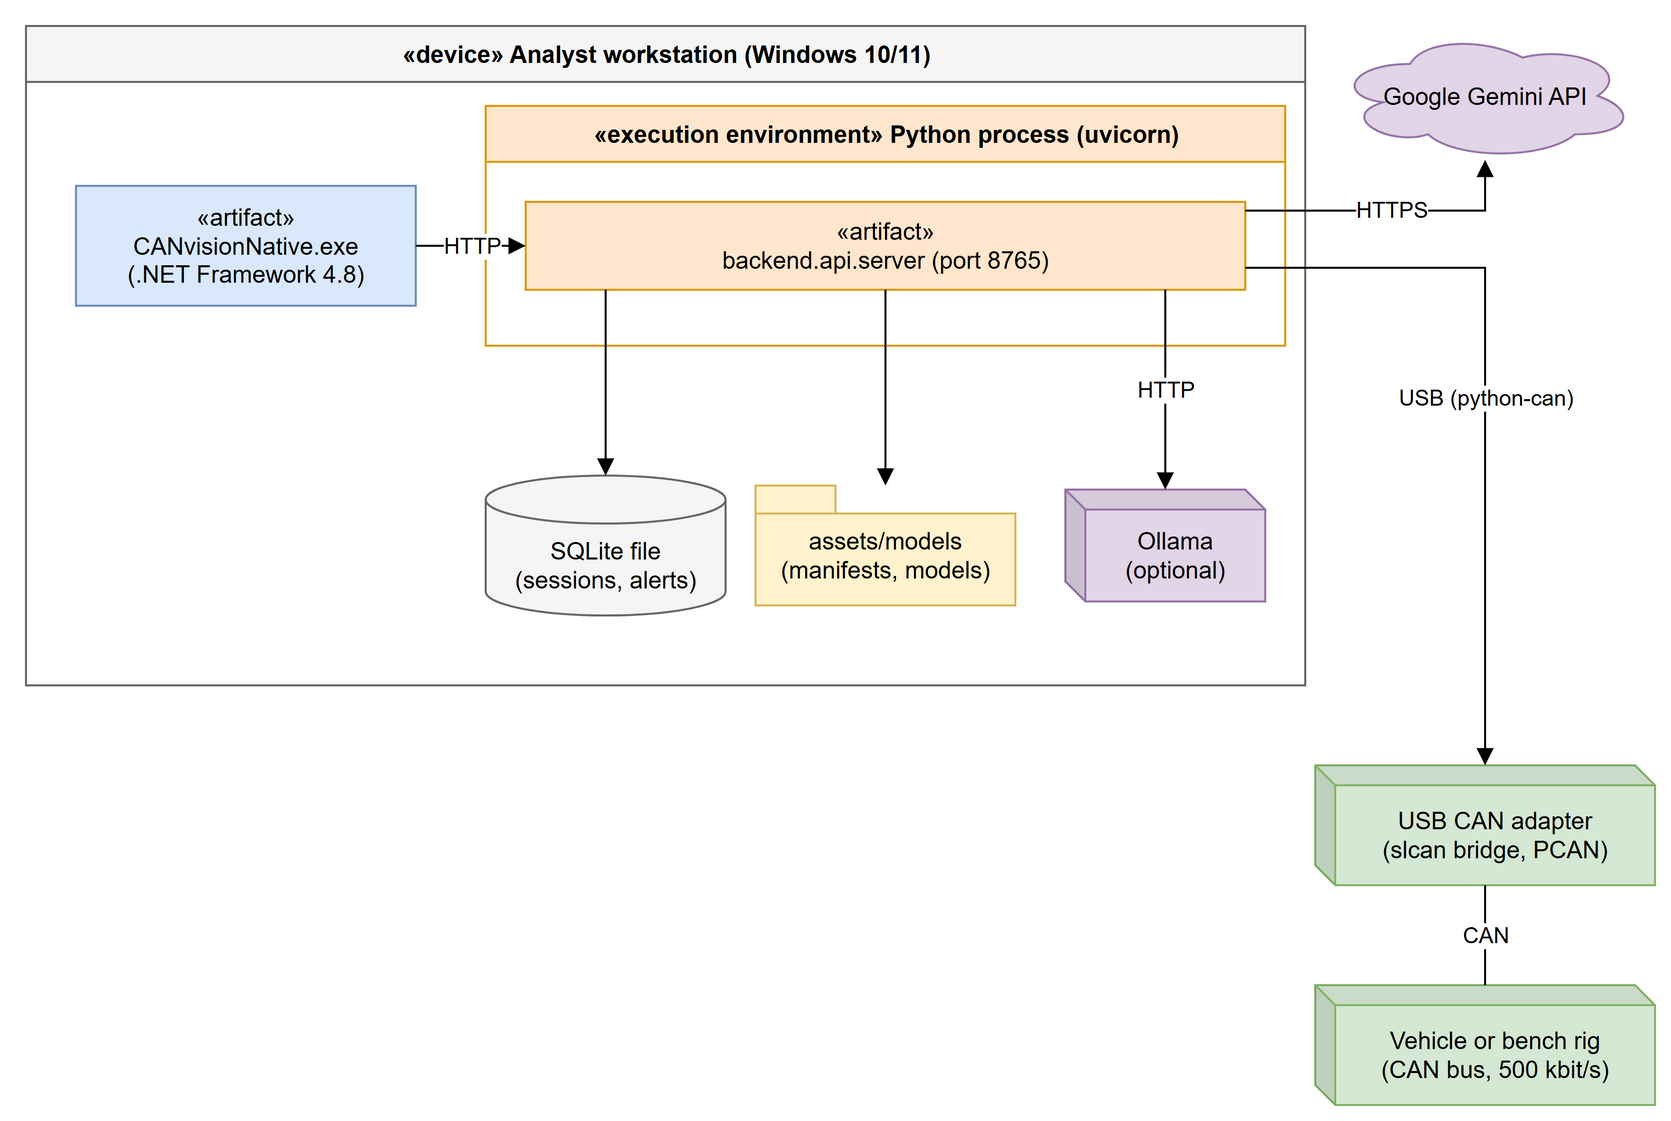
\includegraphics[width=\textwidth]{deployment.png}
\caption[Deployment diagram.]{Deployment diagram: one workstation, with the external \acrshort{llm} and the hardware links.}
\label{fig:deployment}
\end{figure}

\Needspace{631pt}% keep the heading with its float
\section{Analysis model}

\subsection{Domain model}

Figure~\ref{fig:domain-model} shows the concepts of the domain. A \emph{vehicle} may have a \emph{profile}, whose \gls{dbc} files define the \emph{signals} that its frames carry, and a \emph{vehicle model}, made of one \emph{identifier model} per \gls{can} identifier. A \emph{recording} of a vehicle is a sequence of \emph{frames}. A \emph{session}, offline, replay or live, analyses at most one recording with one vehicle model; it counts the frames scored, flagged and unresolved, and produces \emph{alerts}, each of which may receive an \emph{explanation}. A \emph{report} exports one session.

\begin{figure}[H]
\centering
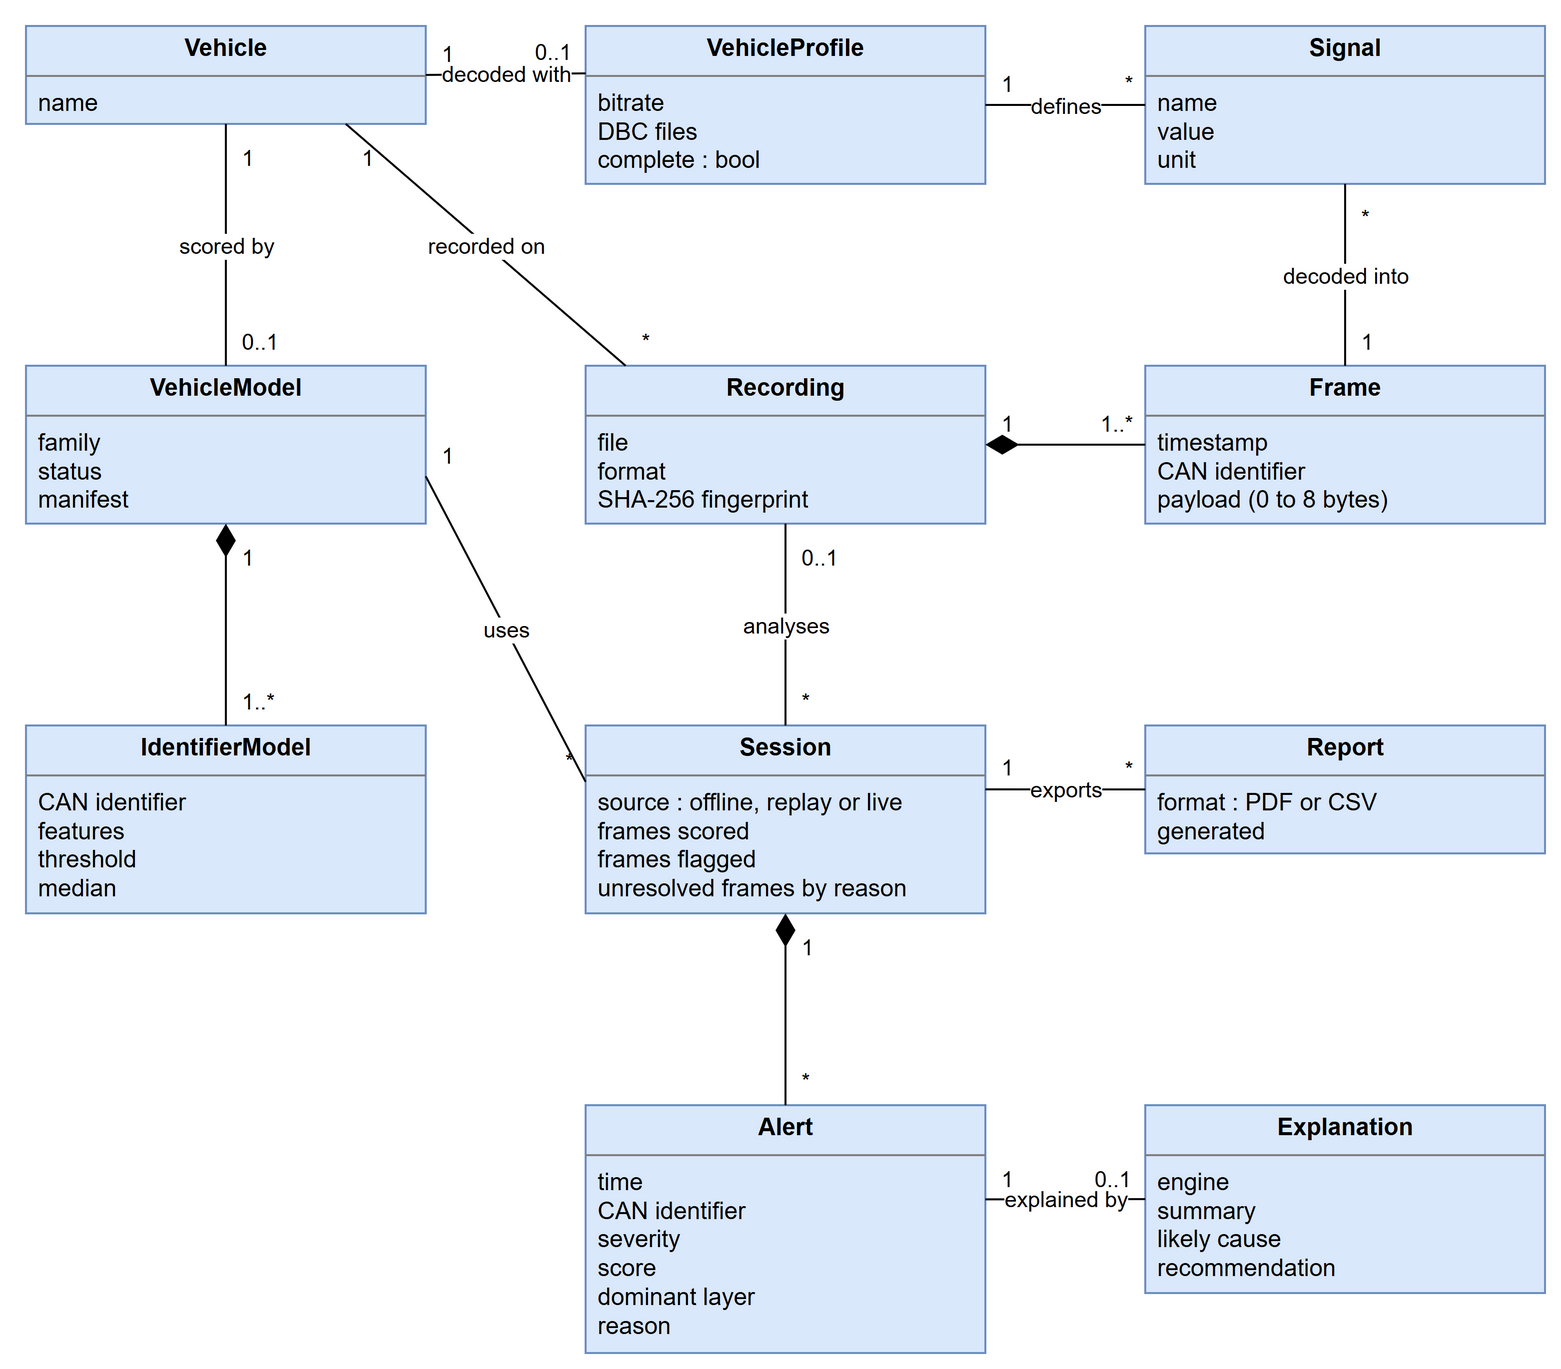
\includegraphics[width=\textwidth]{domain_model.png}
\caption{Domain model of CANvisionNative.}
\label{fig:domain-model}
\end{figure}

\Needspace{555pt}% keep the heading with its float
\subsection{Class diagrams}
\label{sec:class-diagrams}

The class diagrams refine the domain model into the classes of the software, on the backend and on the client side.

Figure~\ref{fig:class-diagram} shows the classes of the detection core of the backend. RealtimeEngine is the single entry point of replay, simulation and live capture; it asks ScoringEngine to combine the layers and, for a vehicle with a final model, its IdModelFamily, loaded from the manifest, for the score of each identifier. The model status resolver decides which model a vehicle may use on each path, and IDSStatistics counts the frames and alerts of a run.

\begin{figure}[H]
\centering
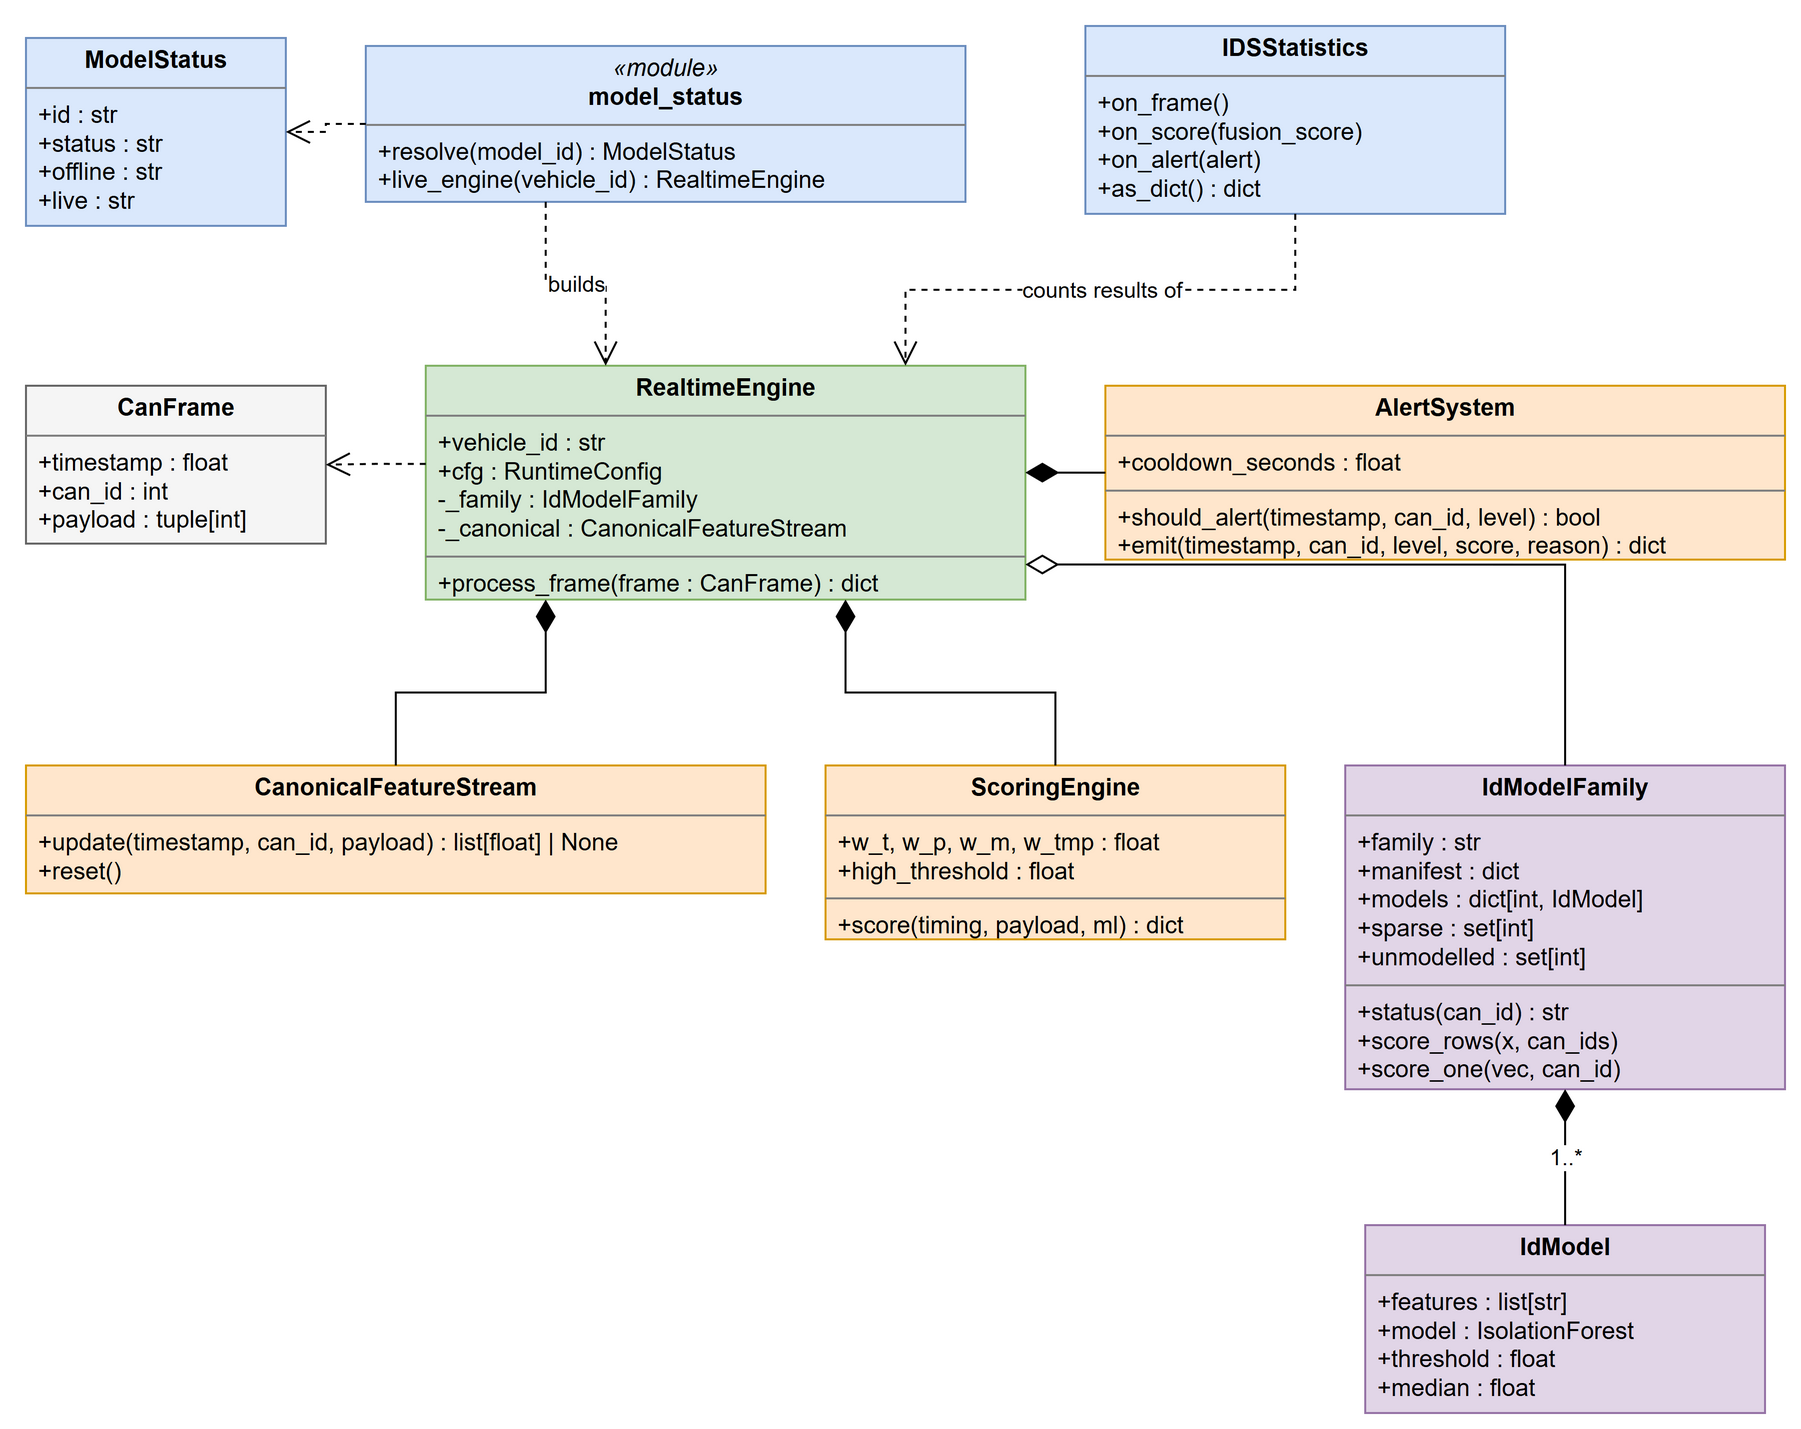
\includegraphics[width=\textwidth]{class_detection_core.png}
\caption{Simplified class diagram of the detection core of the backend.}
\label{fig:class-diagram}
\end{figure}

Figure~\ref{fig:class-client} details the classes of the client. Every screen ViewModel derives from SectionViewModel, which gives it the shared snapshot of the vehicle and access to VehicleDataService. This service owns the state of the session, the alert history and the global state of the application (AppState), and raises events that the screens follow. It calls the backend through PythonApiClient, and CanLogImportService parses a log before an analysis. ModelSelectionService holds the vehicle model chosen by the analyst, and PdfReportBuilder writes the PDF report from the alert list.

\begin{figure}[H]
\centering
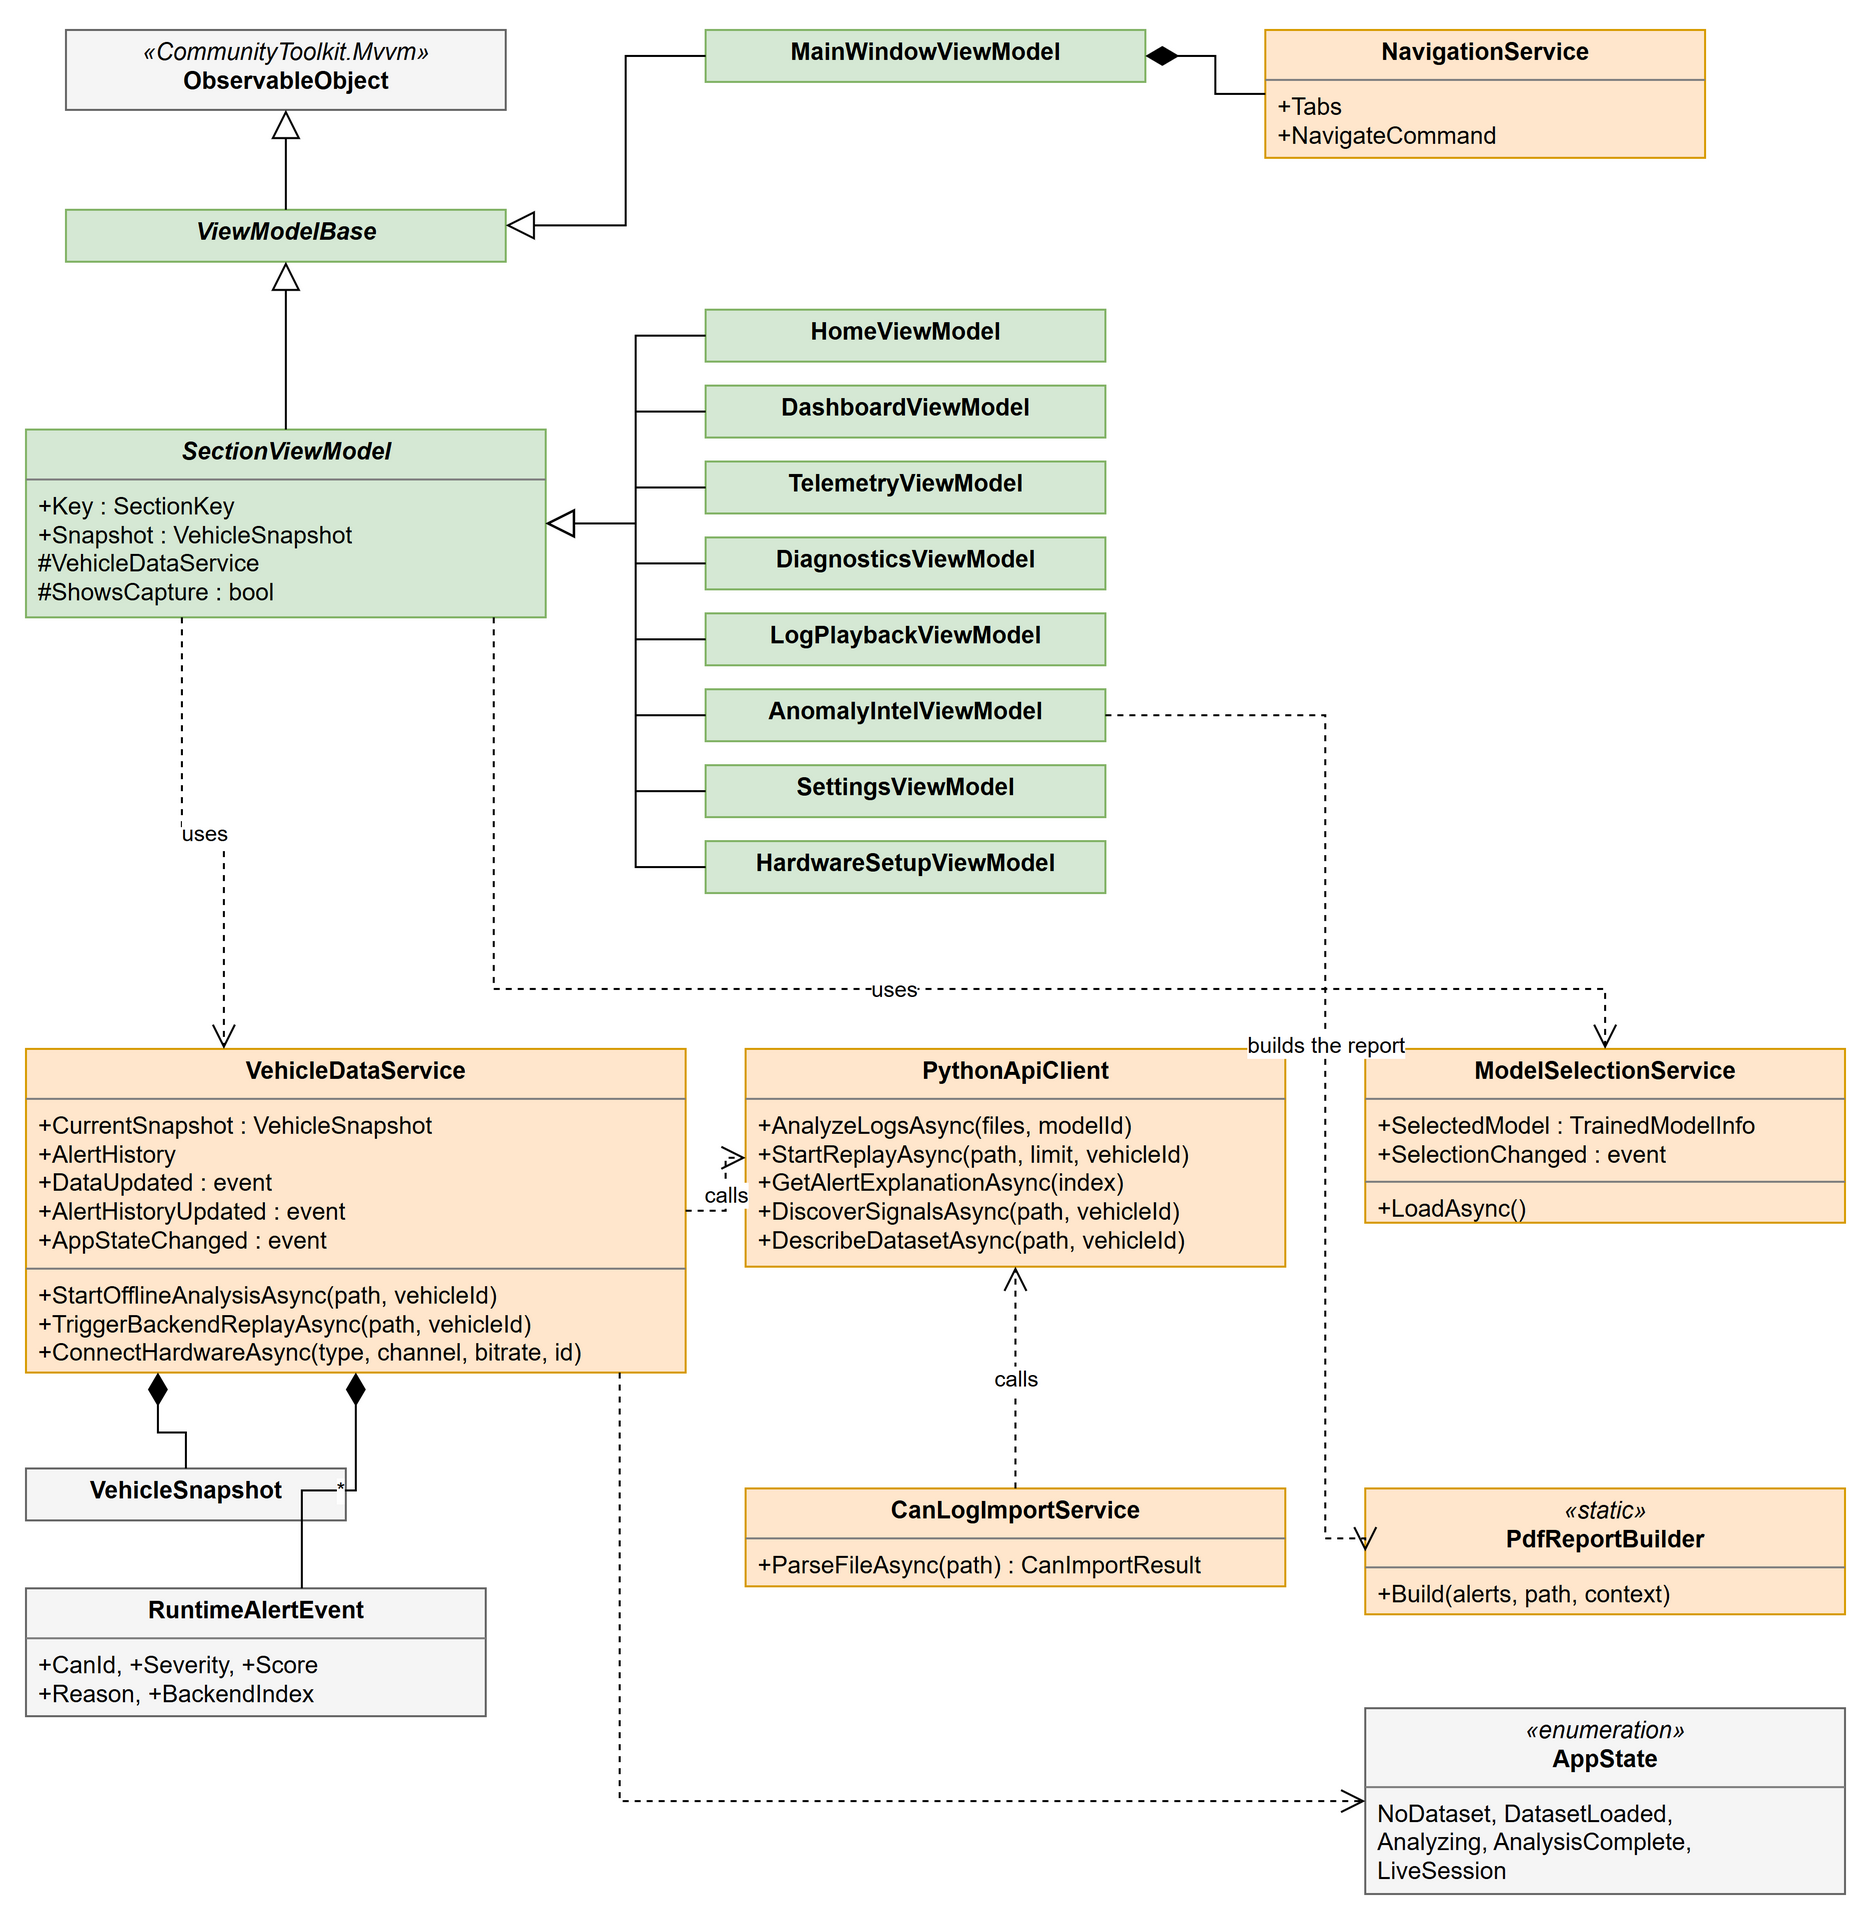
\includegraphics[width=\textwidth]{class_client.png}
\caption{Class diagram of the desktop client.}
\label{fig:class-client}
\end{figure}

\Needspace{464pt}% keep the heading with its float
\subsection{Data model}
\label{sec:data-model}

The backend keeps a small SQLite database (Figure~\ref{fig:data-model}) so that past sessions can be reviewed from a local file. The \code{sessions} table records each session and its source; \code{live\_frames} stores the frames of a session with the result of the detection and an optional label; \code{alert\_history} stores the alerts with their severity, score, reason, temporal pattern and recommended response. The vehicle models are not stored in the database but in model folders, each with its manifest.

\begin{figure}[H]
\centering
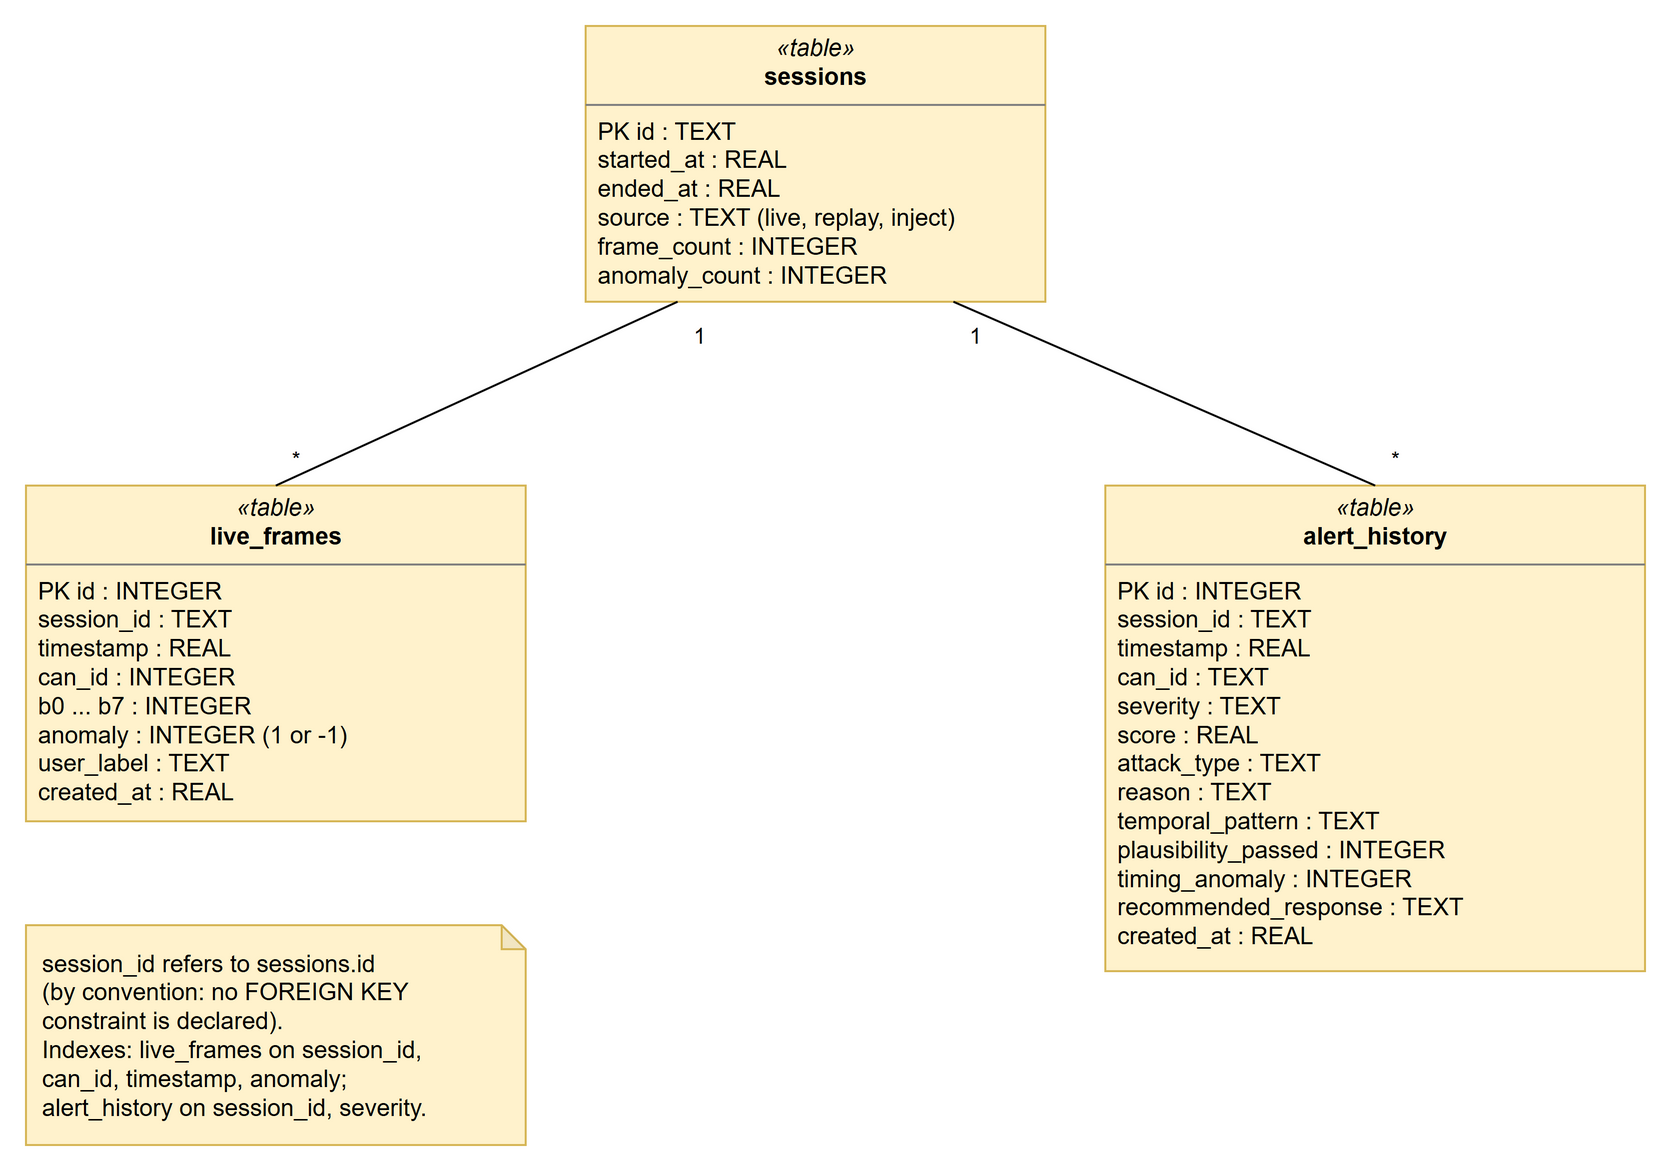
\includegraphics[width=0.9\textwidth]{data_model.png}
\caption{Data model of the SQLite store.}
\label{fig:data-model}
\end{figure}

\section{Dynamic view}

The two sequence diagrams of this section show the key scenarios of a replay and of an explanation. Each object is marked with its nature: \emph{boundary} for the screen the analyst uses, \emph{control} for the objects that coordinate the scenario, and \emph{entity} for the stored data. The messages are numbered in the order in which they are sent; a synchronous call has a filled arrowhead, an asynchronous message an open arrowhead, and a reply a dashed line.

\Needspace{650pt}% keep the heading with its float
\subsection{Life cycle of a replay}
\label{sec:design-replay}

A replay runs in a separate process, so that a long file does not block the backend. It reads the file with the same loader as the offline analysis, so that every format becomes the same stream of (timestamp, identifier, payload) frames, and sends each frame to the same runtime engine as the live and simulated paths. The client follows its progress by polling, and the alerts of the replay are published when it ends so that they can be explained. Figure~\ref{fig:seq-replay} shows this life cycle.

\begin{figure}[H]
\centering
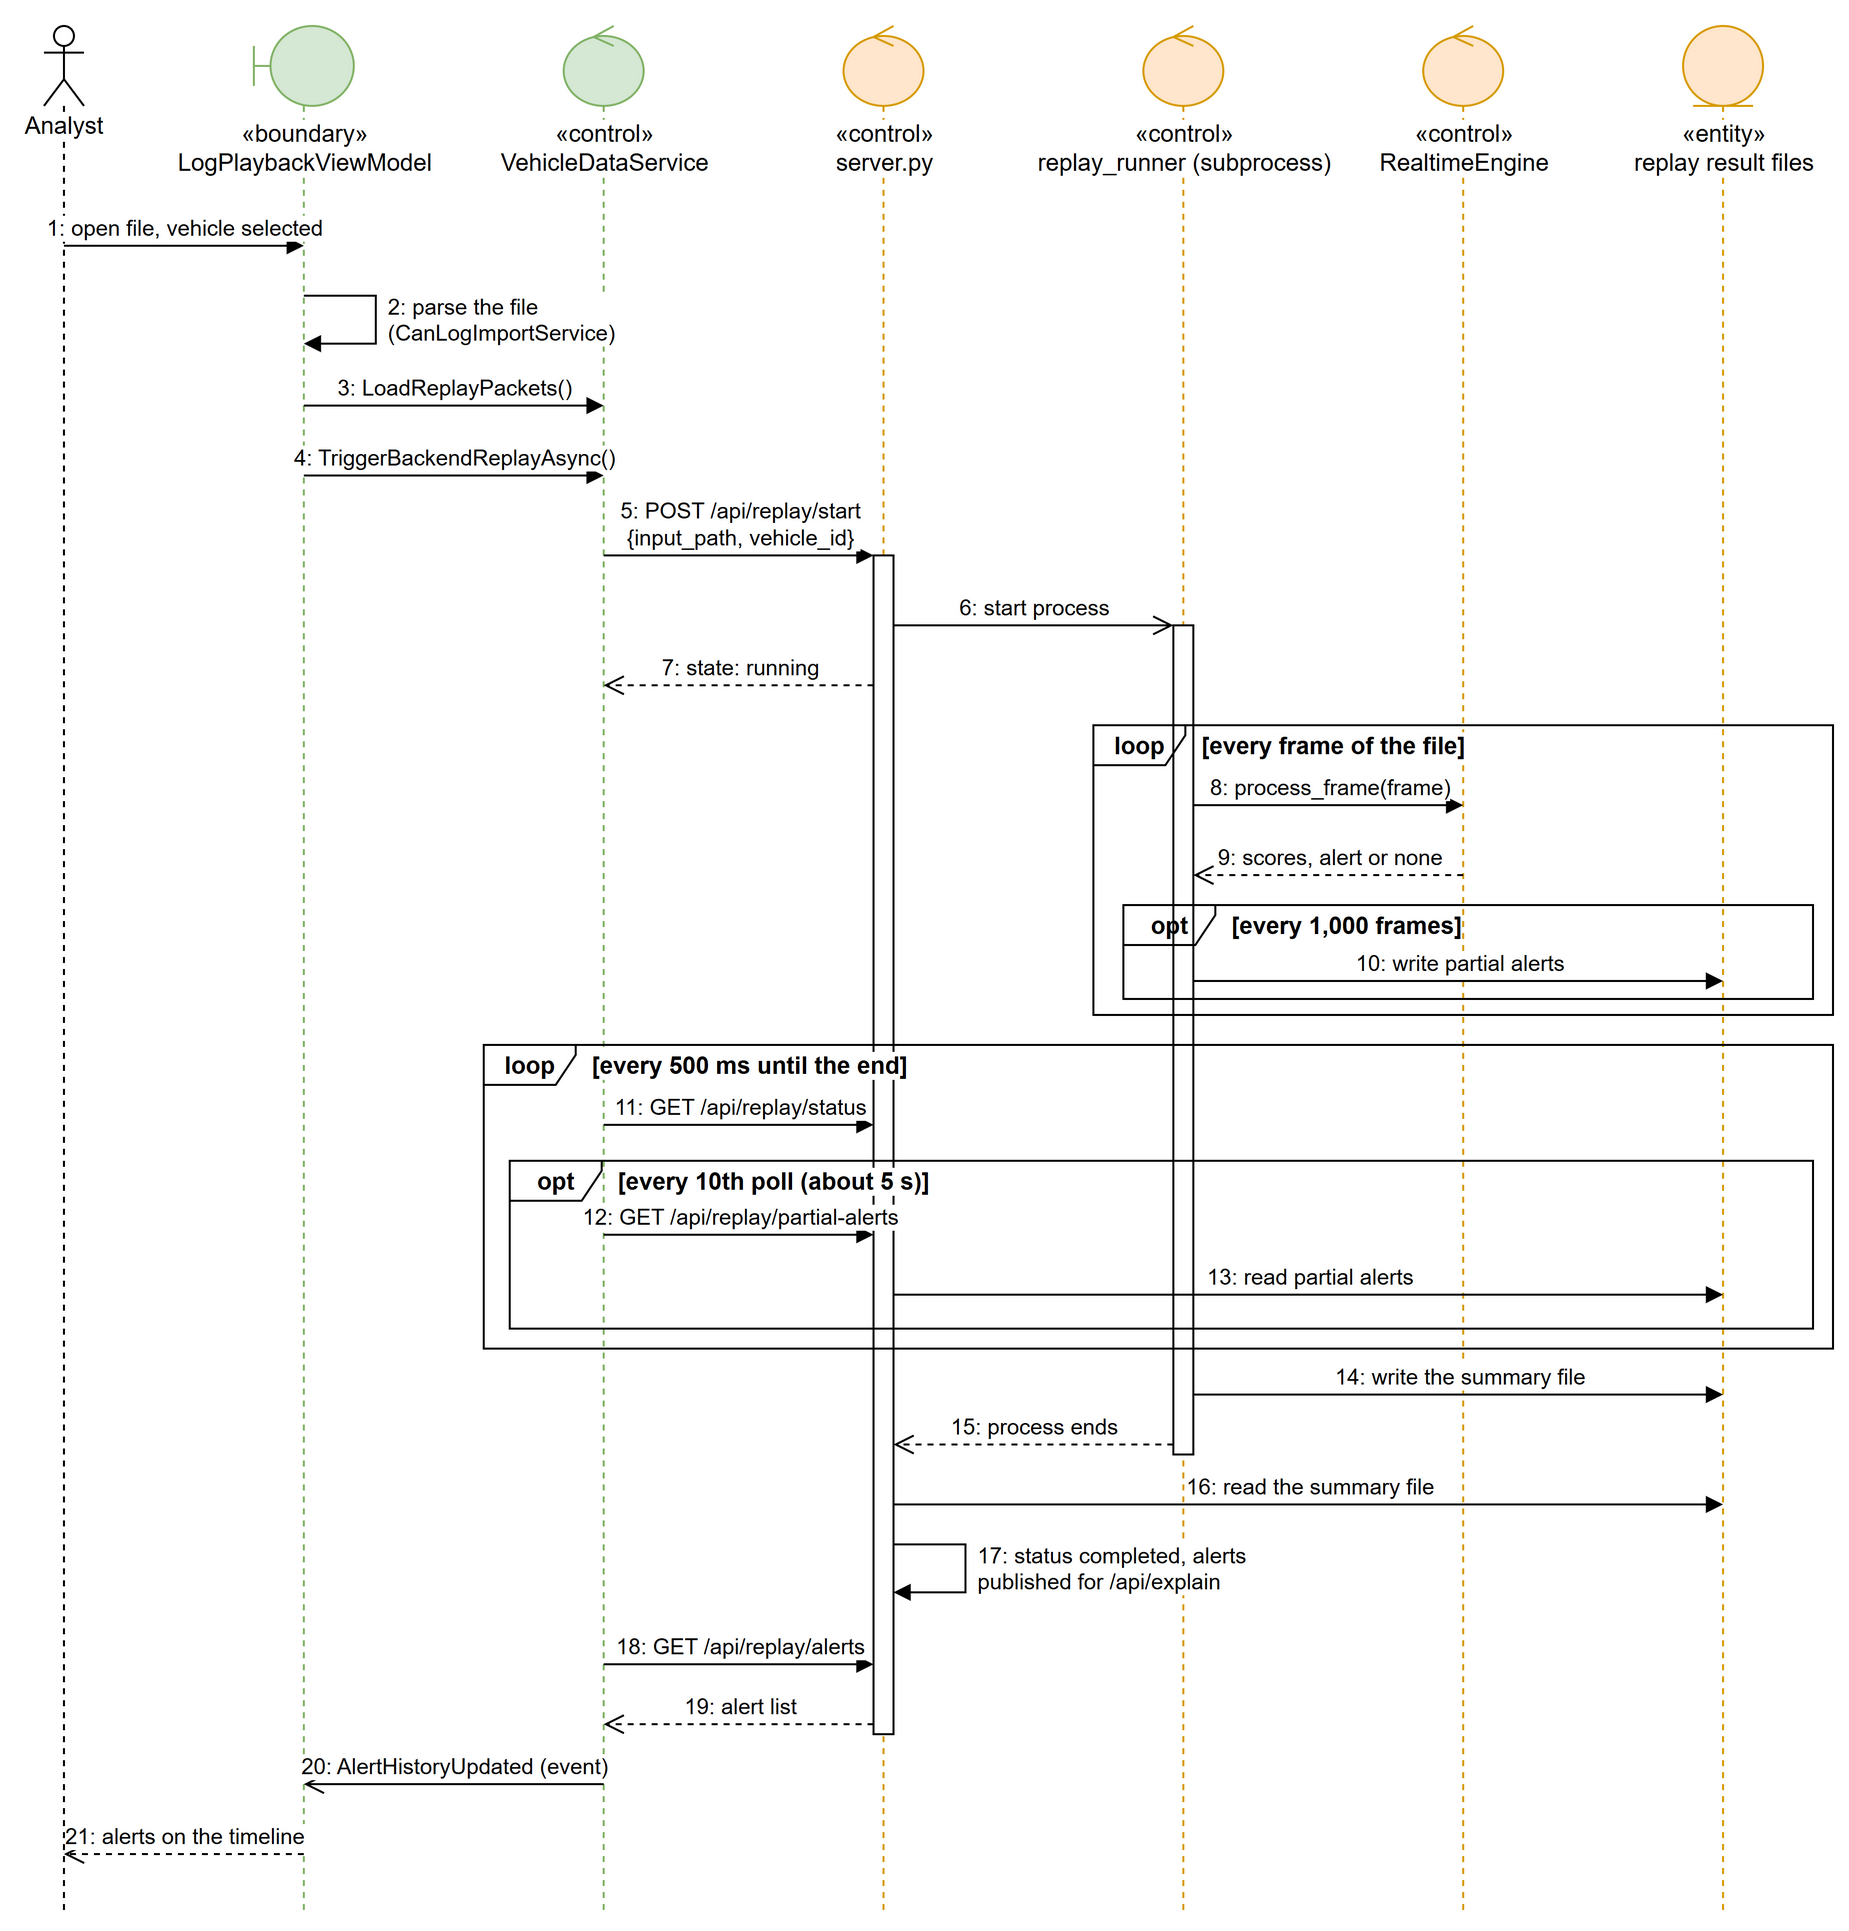
\includegraphics[width=\textwidth]{sequence_replay.png}
\caption[Sequence diagram: life cycle of a replay.]{Sequence diagram: life cycle of a replay, from the client request to the published alerts.}
\label{fig:seq-replay}
\end{figure}

\subsection{Explanation of an alert}
\label{sec:design-ai}

The explanation engine is a supporting feature, not part of detection. It turns the context of an alert into a text an analyst can read: which signal dominated, the likely cause, and what to check. It is called after an alert is raised and never changes a score, a flag or a severity.

When the analyst selects an alert (Figure~\ref{fig:seq-explain}), the backend gathers its context: the measured values and layer scores, the usual behaviour of the identifier, the decoded signals when a \gls{dbc} file exists, known anomaly patterns, similar past cases and, for Gemini, a short web search. Gemini writes the explanation, or a local Ollama model if Gemini cannot be reached; if neither answers, a rule based template fills the same fields from the measured values (NFR6). The engine records the numbers of a model's answer that do not appear in its context, and every answer carries the name of the engine that wrote it, so that a template is never presented as the work of a language model.

\begin{figure}[H]
\centering
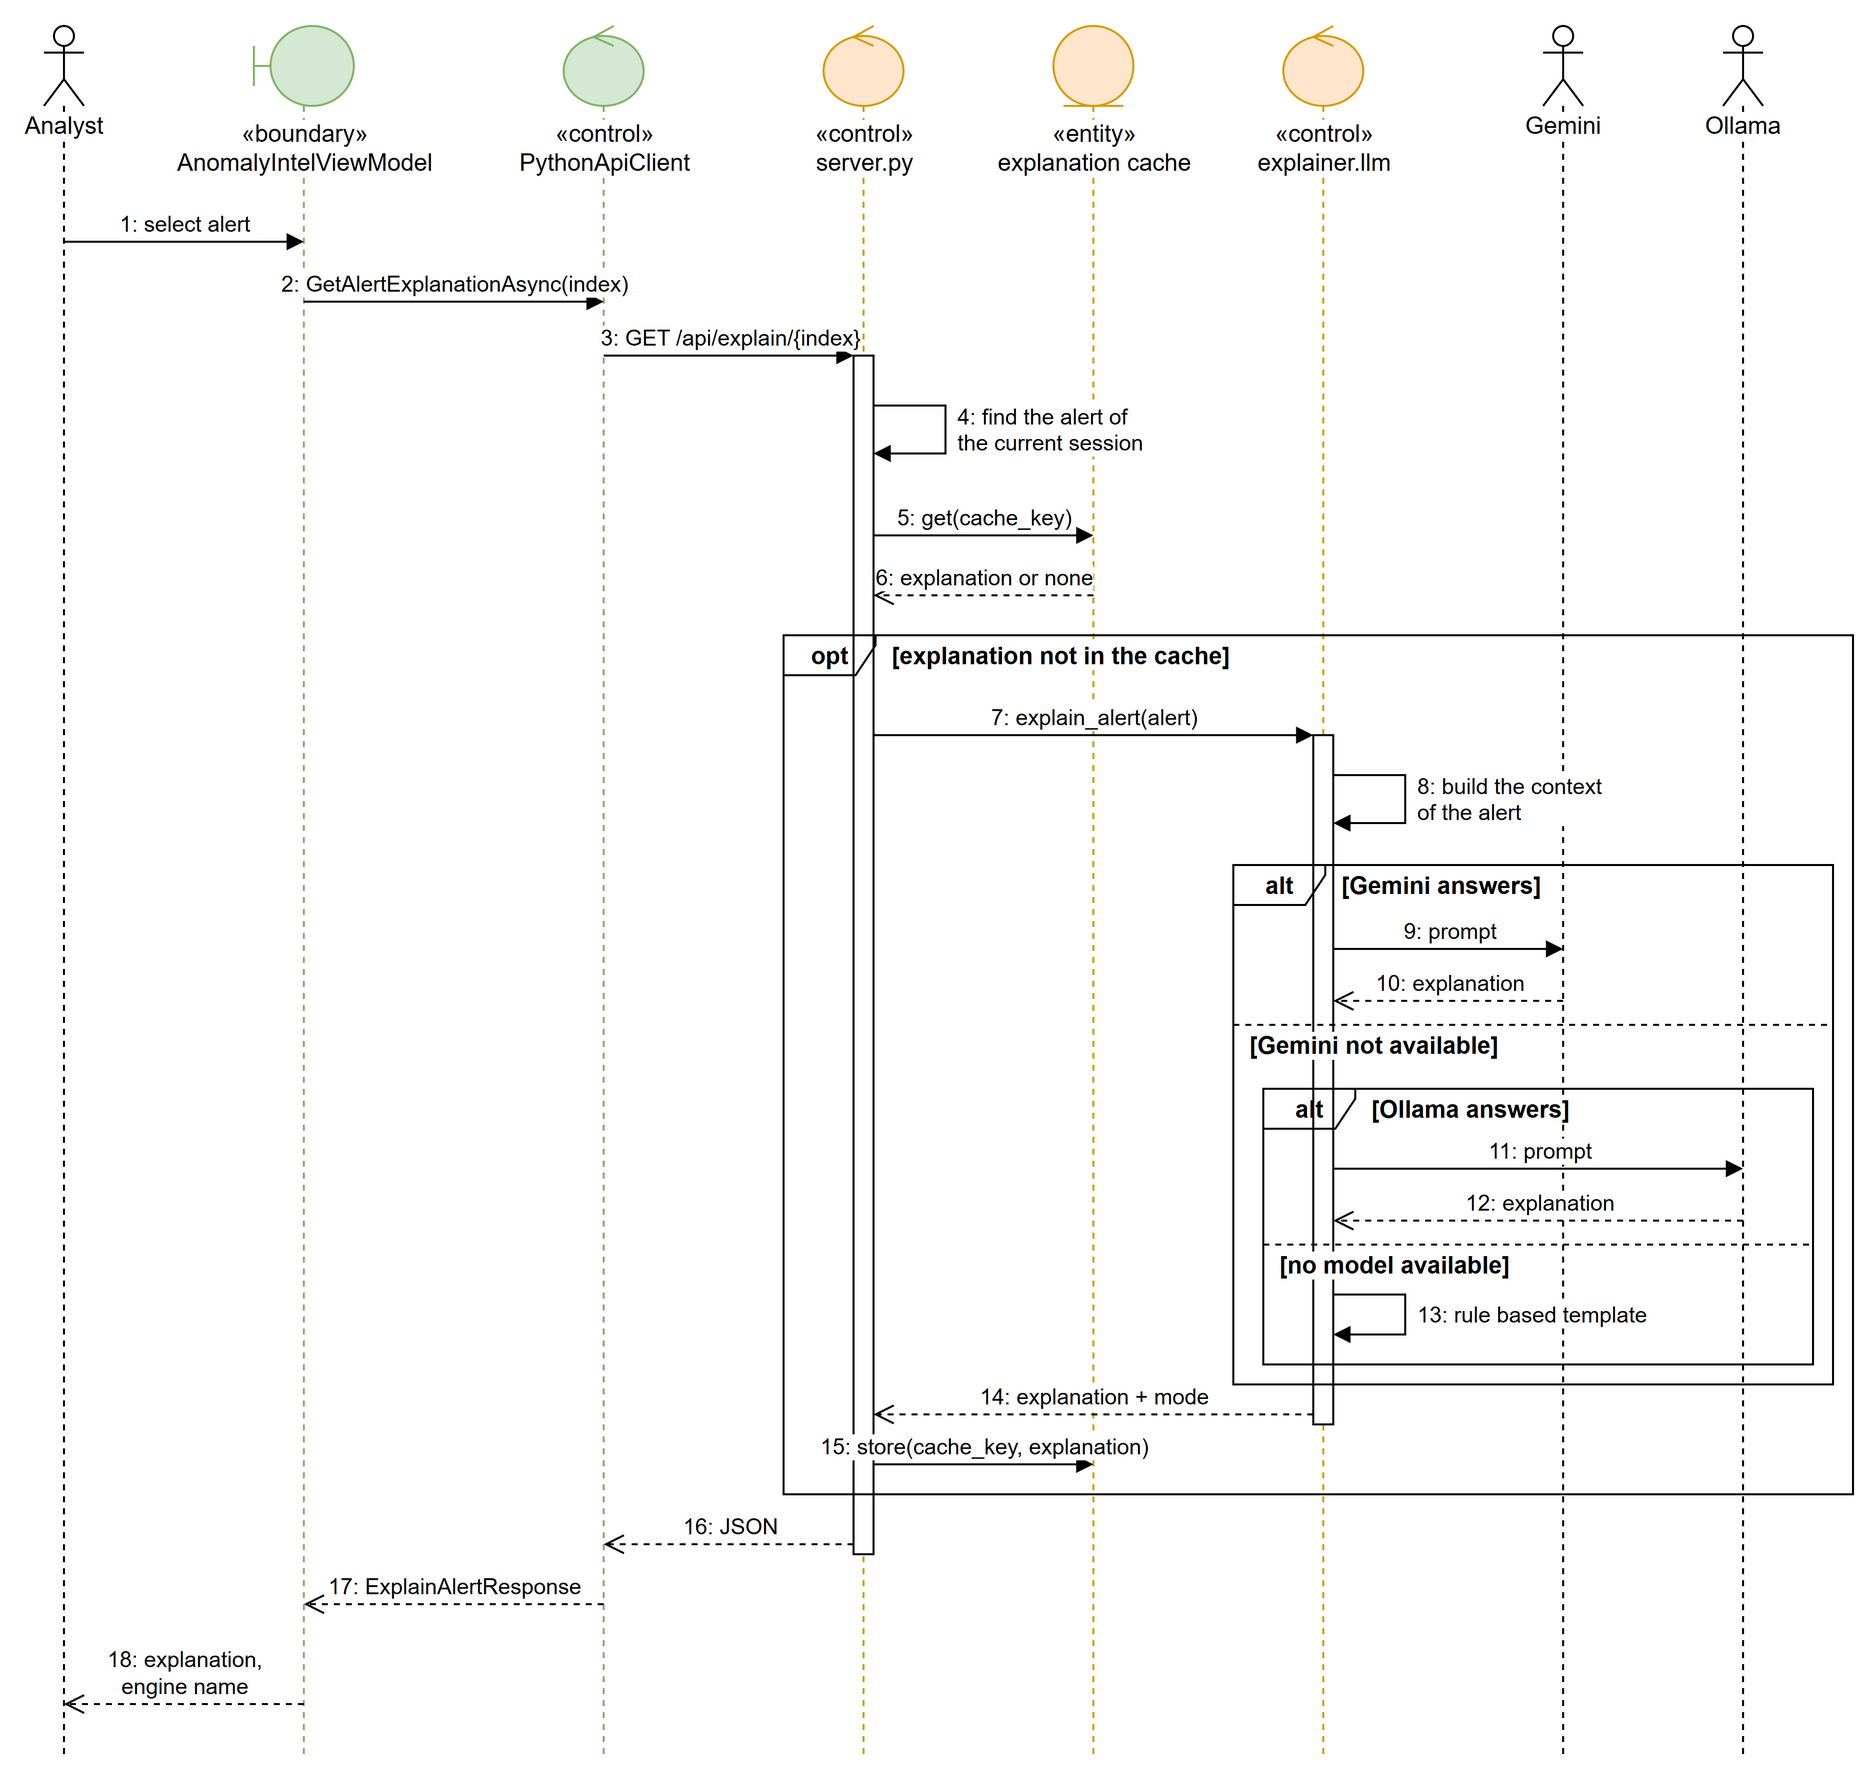
\includegraphics[width=\textwidth]{sequence_explain.png}
\caption{Sequence diagram: requesting the explanation of an alert.}
\label{fig:seq-explain}
\end{figure}

\section{Detection architecture}
\label{sec:design-pipeline}

Frames reach the detection through two paths (Figure~\ref{fig:pipeline}). Replay, simulation and live capture process frames one by one in the runtime engine; the offline analysis receives a whole recording at once. Both use the same features and models, but they turn scores into alerts differently, so the same recording can give different numbers of alerts on each path, and a comparison is only meaningful on one path.

\begin{figure}[H]
\centering
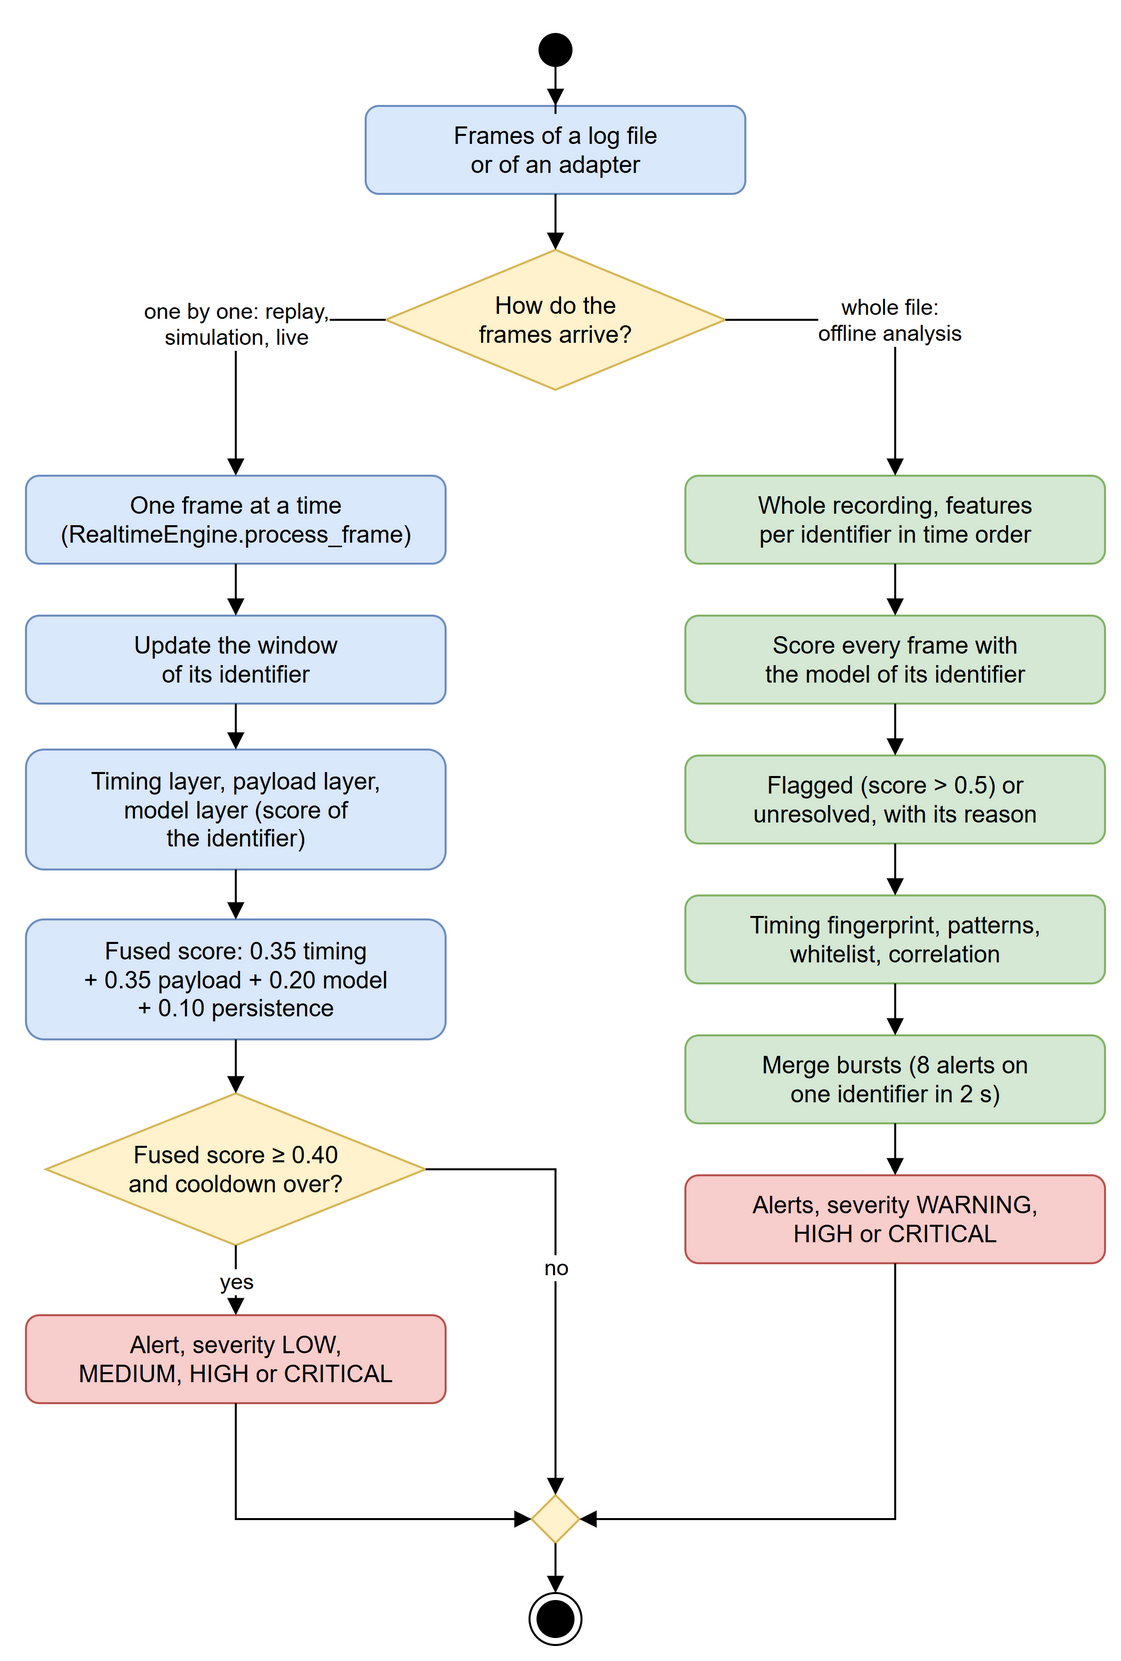
\includegraphics[height=0.66\textheight]{detection_pipeline.png}
\caption[Detection pipeline of the backend.]{Detection pipeline: feature computation per identifier, scoring by the model, additional checks and alerting.}
\label{fig:pipeline}
\end{figure}

\subsection{Frame by frame path (live, simulation, replay)}

For each frame, the runtime engine computes four layer scores:

\begin{itemize}
    \item \textbf{Timing:} The variation of the time between messages of the identifier and its message frequency, whichever is larger, since a regular flood has almost no variation but a very high rate.
    \item \textbf{Payload:} How abruptly the bytes change from one frame of the identifier to the next.
    \item \textbf{Model:} The normalised score given by the model of the vehicle. A frame that no model can score gets no score here, and its status is reported.
    \item \textbf{Persistence:} How many recent frames had a high combined score, so that a sustained anomaly weighs more than a spike.
\end{itemize}

These are combined into one fused score with fixed weights, and Table~\ref{tab:two-paths} gives the alert and severity rules. The weights and thresholds are configuration values, not learned from data.

\begin{table}[H]
\centering
\small
\caption{Scoring and alerting rules of the two detection paths.}
\label{tab:two-paths}
\begin{tabularx}{\textwidth}{|P{2.4cm}|Y|Y|}
\hline
 & \textbf{Frame by frame path (replay, simulation, live)} & \textbf{Offline analysis} \\
\hline
Score & Fused score, each layer from 0 to 2: 0.35 timing + 0.35 payload + 0.20 model + 0.10 persistence & Normalised score of the model, from 0 to 1 \\
\hline
Model call & Every fifth frame of each identifier, the last score reused in between & Every frame \\
\hline
Alert & Fused score $\geq$ 0.40, at most one alert per identifier and second & Each flagged frame (score $>$ 0.5), annotated by the four checks; more than eight alerts on one identifier within two seconds are merged \\
\hline
Severity & LOW $\geq$ 0.30, MEDIUM $\geq$ 0.55, HIGH $\geq$ 0.80, CRITICAL $\geq$ 1.00 & WARNING below 0.55, HIGH $\geq$ 0.55, CRITICAL $\geq$ 0.80; shown in the client as INFO, WARNING and CRITICAL \\
\hline
\end{tabularx}
\end{table}

\subsection{Offline analysis path}

The offline analysis scores every frame with the model of the vehicle. A frame is \emph{flagged} when its score passes the threshold of the model, and a frame that no model can score is counted as \emph{unresolved}, with its reason, instead of normal. Four checks follow: a timing fingerprint of each identifier built from the start of the recording, a frequency analysis that names bursts, frozen payloads and rate spikes, a whitelist of the identifiers seen at the start, and a correlation check between signals linked by a rule, for example a high motor speed with the throttle at zero. Bursts of alerts on one identifier are merged into one summary alert.

\section{Data and machine learning problem framing}
\label{sec:ml-approach}

\subsection{Problem definition}

The learning problem is to decide whether a frame looks like the normal traffic of a given vehicle, without labelled attacks for it. A frame is judged within its own context: a battery voltage message is compared with the usual behaviour of that message, not with the traffic as a whole.

\subsection{Dataset files}
\label{sec:datasets}

All the recordings come from public sources (Figure~\ref{fig:data-logos} and Table~\ref{tab:datasets}); none was bought or obtained under a non disclosure agreement. Only Car-Hacking and the separate attack captures of ROAD carry attack labels.

\begin{figure}[H]
\centering

\includegraphics[height=0.95cm]{css_electronics.pdf}\hspace{0.9cm}

\includegraphics[height=0.95cm]{ornl.pdf}\hspace{0.9cm}

\includegraphics[height=0.95cm]{korea_university.pdf}\hspace{0.9cm}

\includegraphics[height=0.95cm]{github.pdf}
\caption[Sources of the recordings.]{Sources of the recordings: CSS Electronics, Oak Ridge National Laboratory (ROAD), Korea University (Car-Hacking) and GitHub (EV-CANlogs).}
\label{fig:data-logos}
\end{figure}

\begin{table}[H]
\centering
\small
\caption{Dataset files used in the project.}
\label{tab:datasets}
\begin{tabularx}{\textwidth}{|P{2.7cm}|P{3.1cm}|P{2.0cm}|Y|}
\hline
\textbf{Dataset} & \textbf{Vehicles} & \textbf{Format} & \textbf{Use in the project} \\
\hline
CSS Electronics sample data, including the EV Data Pack~\cite{css_evdata} & Kia EV6, Nissan Leaf 2019 & \gls{mf4} & Kia EV6: validation of the first pipeline; Nissan Leaf 2019: training and holdout of a final model \\
\hline
ROAD~\cite{verma2020road} & Real vehicle on a dynamometer & candump log & Ambient recordings only: first corpus, training and holdout of the ROAD ambient model \\
\hline
Car-Hacking~\cite{seo2018gids} & Real vehicle & \gls{csv} with labels & Normal rows only, in the first corpus \\
\hline
EV-CANlogs~\cite{evcanlogs} & Jaguar I-PACE, Kia EV6, BMW i3, MG ZS EV, Tesla and others & \gls{csv}, candump, Vector & Most of the first corpus; training and holdout of the Jaguar I-PACE and Kia EV6 models \\
\hline
Renault Clio log & Renault Clio & candump log & Only to check that no data leaks between sessions \\
\hline
\end{tabularx}
\end{table}

\subsection{Supervised or unsupervised learning}

A supervised approach would need labelled normal and attack frames for every vehicle. Most of the corpus has no labels, the few labelled attacks come from other vehicles and attack methods, a model trained on known attacks is unlikely to recognise a new one, and recording real attacks on every vehicle was not possible. An unsupervised approach only needs the normal traffic of the vehicle, which the corpus has in plenty.

\subsection{Candidate algorithms}
\label{sec:ml-selection}

Table~\ref{tab:ml-comparison} compares the algorithms considered for the anomaly score.

\begin{table}[H]
\centering
\footnotesize
\caption{Candidate machine learning algorithms for the anomaly score.}
\label{tab:ml-comparison}
\begin{tabularx}{\textwidth}{|P{3.1cm}|Y|P{2.6cm}|}
\hline
\textbf{Algorithm} & \textbf{Advantages} & \textbf{Disadvantages} \\
\hline
Isolation Forest~\cite{liu2008isolation} & Fast to train, no distance computation, no assumption on the distribution; suited to numeric tabular features. & Harder to read than a rule; needs a decision threshold. \\
\hline
One Class SVM~\cite{scholkopf2001estimating} & Well studied, with a clear geometric meaning. & Training cost grows fast with the data; sensitive to its kernel. \\
\hline
Local Outlier Factor (LOF)~\cite{breunig2000lof} & Captures local differences of density. & Keeps the training data; its prediction cost grows with it. \\
\hline
DBSCAN~\cite{ester1996density} & Finds clusters of any shape without fixing their number. & Gives no score for a new point. \\
\hline
Random Forest (supervised) & Very accurate with labelled data. & Needs labelled attacks for each vehicle. \\
\hline
Autoencoder & Can model complex normal patterns. & Needs more data and tuning; harder to explain. \\
\hline
K-Means~\cite{macqueen1967methods} & Simple and fast. & Not an anomaly detector by itself. \\
\hline
\end{tabularx}
\normalsize
\end{table}

\subsection{Choice of Isolation Forest}

The algorithm had to learn from normal data only, give a result an analyst can understand (``how unusual is this frame''), and score a frame quickly enough for replay and live capture. Isolation Forest meets the first two criteria by construction: it is trained on normal traffic, and an anomalous point is isolated after fewer random splits. DBSCAN was set aside because it gives no score for a new frame, the autoencoder because it is harder to explain and debug, and the supervised Random Forest because no labelled attacks exist for our vehicles. LOF and the One Class SVM remained credible alternatives, so we planned to measure them against Isolation Forest once the final models existed, on the same data and under the same rule.

\section{Architecture baseline}
\label{sec:baseline}

The elaboration phase ended with an executable architecture, delivered by milestone M1, the live foundation. It connected the two programs end to end before any vehicle model existed: the client started and stopped a live session through new \gls{api} endpoints, the backend scored a simulated stream frame by frame in the runtime engine, an alert reached the client, and the Dashboard charted the fused score of the last frames. A smoke test checked this chain, from the simulated data to the scoring, the alert and the update of the Dashboard.

This baseline reduced three risks of Table~\ref{tab:risks}. Live capture would only differ from replay and simulation by its transport, since all three feed the same runtime engine (R1). Every source would enter the engine as the same frame representation (R7). And the client and the backend were shown to work together through the \gls{api}, so that the following iterations could add features on both sides without changing how they communicate.

\section{Conclusion}

This chapter presented the technical choices, the architecture of the client and the backend, the domain and data models, the dynamic view of a replay and of an explanation, the two detection paths, the framing of the machine learning problem, and the architecture baseline of the elaboration phase. The next chapter presents the four iterations of the construction phase.
